\documentclass[lang=cn,10pt]{elegantbook}

\title{计算机系统(2)实践手册}
% \subtitle{}

\author{ACM班课程助教}
\institute{ACM班,上海交通大学}
\date{2024-2025春季学期}
\version{1.1.1}
% \bioinfo{}{}

\definecolor{codebg}{rgb}{0.95,0.95,0.95}
\lstset{
    backgroundcolor=\color{codebg},
    basicstyle=\ttfamily\footnotesize,
    breaklines=true,
    frame=single,
    captionpos=b
}
\extrainfo{}

\setcounter{tocdepth}{3}

% \logo{logo-blue.png}
\cover{cover.jpg}

% 本文档命令
\usepackage{array}
\newcommand{\ccr}[1]{\makecell{{\color{#1}\rule{1cm}{1cm}}}}

% 修改标题页的橙色带
% \definecolor{customcolor}{RGB}{32,178,170}
% \colorlet{coverlinecolor}{customcolor}

\begin{document}

\maketitle
\frontmatter

\tableofcontents
\chapter*{实践任务的背景}

在21世纪20年代,机器学习的极具发展、大模型的快速迭代使得操作系统相关的内容成为“不受大家待见”的东西。
学术界急速转向机器学习系统相关系统使得大家对于传统硬核的操作系统失去了兴趣。
不仅班级内发生了转向,大多数实验室也在这一期间放弃原有传统系统研究而转向新兴与大模型结合的系统研究。
为了适应这一潮流,对于对计算机系统没有兴趣的同学,助教们经过讨论认为需要将重点放在“如何使用好操作系统”和“如何理解操作系统的能力”两个部分。
为此,助教们结合2019、2020、2021、2022级日常作业的内容,将小作业实践总结的目标进行整合,整理出了这一版实践的目标手册。

由于时间仓促,这一版本内容相对比较单薄。期待同学们在作业发展的过程中不断迭代增加内容。

第一版实践手册牵头讨论和实践的同学是郑文鑫(2017)、王鲲鹏(2022)、房诗涵(2022)、徐子绎(2022)、潘屹(2022)。
\mainmatter

\chapter{总述}
\section{作业内容}
本系列作业旨在引导大家通过修改Linux内核的实现感受操作系统的功能。
作业具体包括以下6个大类:启动、系统调用与特权态执行、内存管理、文件系统、网络与外部设备、安全。
每个大类进一步根据难度和内容分为基础、实践、设计、综合。前三部分的内容如表\ref{fig:intro:all}所示。
综合部分的选题每一个选题横跨两个子项目,内容和目标如表\ref{fig:intro:mixed}所示。

\begin{table}[htbp]
\centering

\caption{分项内容}
\label{fig:intro:all}
\begin{tabular}{c|c|c|c}

\hline
分项                                                 & 基础      & 实践  & 设计         \\ \hline
系统启动         & Read ACPI Table     & Hack ACPI Table & UEFI运行时服务 \\ \hline
\begin{tabular}[c]{@{}c@{}}系统调用\\ 特权态\end{tabular} & 用户定义的系统调用     & vDSO & 无需中断的系统调用     \\ \hline
内存管理                                               & 页表和文件页      & 内存文件系统 & 内存压力导向的内存管理        \\ \hline
文件系统                                               & inode和扩展属性管理     & FUSE & 用户空间下的内存磁盘       \\ \hline
\begin{tabular}[c]{@{}c@{}}网络\\ 外部设备\end{tabular}  & tcpdump和socket管理  & NCCL & DPDK       \\ \hline
% \begin{tabular}[c]{@{}c@{}}安全\\ 虚拟化\end{tabular}  & 常见的溢出攻击和侧信道 & 虚拟机调用Hypercall & 虚拟机内存访问加速        \\ \hline
\end{tabular}
\end{table}


\begin{table}[htbp]
\centering

\caption{综合部分分项内容}
\label{fig:intro:mixed}
\begin{tabular}{c|c}
\hline
项目              & 涉及分项         \\ \hline
使用RDMA的远程内存Swap & 内存管理、网络与外部设备 \\ \hline
用户程序嵌入内核执行 & 系统调用、内存管理 \\ \hline
内核空间下的内存磁盘 & 内存管理、文件系统 \\ \hline
机密虚拟机Trapless的宿主协同内存管理 & 内存管理、安全与虚拟化 \\ \hline

\end{tabular}

\end{table}

\section{作业安排(初步)}

在本学期的作业中,我们将会定期安排大家进行习题课完成答疑和基本环境配置。小作业的初步计分规则如下(满分100分),正式发布在3月1日。

\begin{enumerate}
    \item 基础部分:每个分项5分,共30分,必选;
    \item 实践部分:每个分项10分,共60分;
    \item 设计部分:每个分项15分,共90分;
    \item 综合部分:每个分项50分,选一个共50分。
\end{enumerate}

作业层级之间存在关联,即实践部分的内容可能会依赖基础部分的内容,设计部分的内容可能会依赖实践部分的内容,综合部分的内容可能会依赖设计部分的内容。因此,建议大家按照顺序完成作业。
分数的设定同样存在层级关联,实践部分需要基础部分完全完成才可以计算,设计部分需要至少完成2个实践部分才可以计算,综合部分需要至少完成1个设计部分才可以计算。
综合部分可能需要用到特别的硬件,如果需要使用特殊的硬件请联系助教。

\paragraph*{诚信原则}
如果出现以下情况,将会扣分:
\begin{enumerate}
    \item 某一项作业与他人完全一致(即使是两人都是用大模型生成):计小作业0分。
    \item 某一项作业疑似使用大模型生成且没有对代码的合理解释:计该项作业0分。
\end{enumerate}

\paragraph*{作业提交}
为了方便大家更加使用符合自己使用习惯的内核,我们允许使用任何Linux 5.x.x的内核版本完成作业。(不建议使用6.0以及更高版本,也不建议使用5.0之前的4.x版本)。请在4月15日前提交你的基础版本号。
对于每一个作业,你需要提交按照作业要求上载明的内容(部分的作业子项要求报告)和对应与base版本的diff文件。提交的文件格式为pdf和patch文件。
所有作业的截止时间均为本学期16周周日晚上23:59,但是自第8周开始,你可以提前提交作业(Code Review仍然安排在16周),提前提交作业不会有额外的加分。

\paragraph*{Code Review}
Code Review将会在16周进行,具体时间和地点将会在之后公布。Code Review的内容将会包括对你的代码的评价和对你的报告的评价。Code Review的分数将会占到你分项的30\%。
\textbf{你不应当认为Code Review是容易获得满分的。}

\paragraph*{额外加分}
我们鼓励大家通过向本Repo提交PR来提高你的分数。每一个PR将会有0.1至2分不等的加分(加小作业部分分),分数取决于表述的质量和作用。
PR的内容可以是对本Repo的文档的修正,对作业的补充,对作业的环境配置提供的建议等等。
修正错别字、表述错误至多可以提交10次,每次0.1分。
对作业描述的补充、环境配置按照书写的质量给分。
其余类型的PR提交后请联系助教确认加分。
要求释疑很大概率不会获得加分。
重复提交不给分(重复修复同一个错别字、重复给出相似的作业描述补充等),按照PR的编号决定加分对象。加分给编号较小的人。
最终加分不超过20分。
\chapter{项目环境准备}

\section{基准代码}
本系列的基准代码规则如下:
\begin{enumerate}
    \item \textbf{Linux}: 任何体系结构下高于5.10.20版本的Linux内核都是可行的选项,你可以从\url{https://www.kernel.org/}中选择合适的版本。对于\texttt{initramfs},你可以选择任何一个发行版。如果你选择直接使用qcow或者其他完全预制好的Ubuntu镜像,你需要手动在内部更换内核以确保你的代码能够生效。
    \item \textbf{QEMU}: 版本>=7。
    \item \textbf{EDK2}: 跟随\url{https://github.com/tianocore/edk2}选择合适的版本。其中Ubuntu\_GCC5并不意味着GCC版本必须是5。
\end{enumerate}

\section{在QEMU中启动Linux镜像}
\begin{remark}
简单起见你可以直接使用预制作好的\texttt{qcow} Ubuntu镜像作为磁盘镜像由qemu直接引导,具体教程:\url{https://documentation.ubuntu.com/public-images/en/latest/public-images-how-to/launch-qcow-with-qemu/}。如果你选用这个方案,你只需要确保QEMU正常安装即可。
\end{remark}

\begin{remark}
    本区域中.x.x部分请填入自己对应的版本号。
\end{remark}



\subsection{QEMU安装(二选一)}
\subsubsection{软件包安装}
\begin{lstlisting}[language=bash]
sudo apt-get install qemu-system-x86
qemu-system-x86_64 --version
\end{lstlisting}

\subsubsection{源码编译安装}
\begin{lstlisting}[language=bash]
# 安装依赖
sudo apt-get install git libglib2.0-dev libfdt-dev libpixman-1-dev zlib1g-dev ninja-build

# 下载编译
mkdir ~/kvm && cd ~/kvm
wget https://download.qemu.org/qemu-7.2.0.tar.xz
tar -xf qemu-7.2.0.tar.xz
cd qemu-7.2.0
./configure --target-list=x86_64-softmmu
make -j$(nproc)
\end{lstlisting}

\subsubsection{常见依赖问题}
\begin{itemize}
    \item \textbf{ERROR: Cannot find Ninja} → 执行 \texttt{sudo apt install ninja-build}
    \item \textbf{ERROR: glib-2.56 required} → 执行 \texttt{sudo apt install libglib2.0-dev}
    \item \textbf{Dependency "pixman-1" not found} → 执行 \texttt{sudo apt install libpixman-1-dev}
\end{itemize}

\subsection{Linux内核编译}
\begin{lstlisting}[language=bash]
# 安装依赖
sudo apt-get install git fakeroot build-essential ncurses-dev xz-utils libssl-dev bc flex libelf-dev bison 
mkdir ~/kernel && cd ~/kernel
wget https://git.kernel.org/pub/scm/linux/kernel/git/stable/linux.git/snapshot/linux-5.x.x.tar.gz
tar -xf linux-5.x.x.tar.gz
cd linux-5.x.x

make defconfig    # 使用默认配置
make -j$(nproc)   # 开始编译
\end{lstlisting}

\textbf{编译输出文件}: \texttt{arch/x86/boot/bzImage}

在编译过程中,可能会发生编译错误的情况。这可能是 GCC 版本过高导致的。这里给出一种可行的组合: Linux-5.19.17, 使用 GCC-12 进行编译,操作如下:

\begin{lstlisting}[language=bash]
sudo apt install gcc-12 g++-12 # 安装gcc-12
sudo update-alternatives --install /usr/bin/gcc gcc /usr/bin/gcc-12 70
sudo update-alternatives --install /usr/bin/g++ g++ /usr/bin/g++-12 70 # 切换 gcc 默认版本
\end{lstlisting}
经过这些操作后,应该可以正常编译 Linux 内核了。

\subsection{BusyBox}
\subsubsection{直接安装}
直接使用你的开发环境自带的包管理器安装busybox,然后在后面制作initramfs的过程中添加这两步:

先把busybox拷贝进initramfs:
\begin{lstlisting}[language=bash]
cp $(which busybox) "${INITRAMFS_DIR}/bin/busybox"
\end{lstlisting}

然后在系统启动脚本里添加:
\begin{lstlisting}[language=bash]
/bin/busybox --install -s /bin
\end{lstlisting}
\subsubsection{手动编译安装}
这里可以采用其他发行版(例如Ubuntu发行版等)。
\begin{lstlisting}[language=bash]
mkdir ~/kvm && cd ~/kvm
wget https://busybox.net/downloads/busybox-1.x.x.tar.bz2
tar -xf busybox-1.x.x.tar.bz2
cd busybox-1.x.x

# 配置命令
make menuconfig
# 选中: Settings > Build Options > [*] Build static binary
# 取消: Shells > [ ] Job control

make -j$(nproc) && make install
\end{lstlisting}
如果在编译过程中出现错误( TCA\_CBQ\_MAX undeclared ),一种解决方式是直接删除出错的 “tc.c” 文件。之后就可以正常编译了(版本 1.32.0 可以用此方法解决)。

\subsection{EDK2编译}
EDK2的可编译源码在git submodule里,因此相对简单可靠的方式就是直接按照官网所说的那样:
\begin{lstlisting}[language=bash]
git clone -b stable/202408 https://github.com/tianocore/edk2.git
cd edk2
git submodule update --init
\end{lstlisting}
在编译之前,需要在系统里安装一些基础的包(例如base-devel uuid、nasm、acpica),然后就可以编译BaseTools。
\begin{lstlisting}[language=bash]
source edksetup.sh
make -C BaseTools -j$(nproc)
\end{lstlisting}
然后编辑\texttt{Conf/target.txt}(参考\url{https://github.com/tianocore/tianocore.github.io/wiki/How-to-build-OVMF}):
\begin{lstlisting}
ACTIVE_PLATFORM       = OvmfPkg/OvmfPkgIa32X64.dsc
TARGET_ARCH           = IA32 X64
TOOL_CHAIN_TAG        = GCC5
\end{lstlisting}
最后,执行:
\begin{lstlisting}[language=bash]
build
\end{lstlisting}
然后就可以在\texttt{Build/Ovmf3264/DEBUG\_GCC5/FV/}目录找到\texttt{OVMF\_CODE.fd}和\texttt{OVMF\_VARS.fd}两个编译出的OVMF文件。(这里的Ovmf3264和DEBUG\_GCC5和编译选项有关,也是在\texttt{Conf/target.txt}里面配置。)

\subsection{制作initramfs}
\subsubsection{创建启动脚本}
\begin{lstlisting}[language=bash, language=bash, showstringspaces=false]
cd busybox-1.x.x/_install/
mkdir -p proc sys dev tmp
echo -e '#!/bin/sh\nmount -t proc none /proc\nmount -t sysfs none /sys\nmount -t tmpfs none /tmp\nmount -t devtmpfs none /dev\necho "Hello Linux!"\nexec /bin/sh' > init
chmod +x init
\end{lstlisting}

\subsubsection{打包文件系统}
\begin{lstlisting}[language=bash]
find . -print0 | cpio --null -ov --format=newc | gzip -9 > ../initramfs.cpio.gz
\end{lstlisting}

\subsection{启动QEMU}
\subsubsection{图形界面启动}
\begin{lstlisting}[language=bash]
qemu-system-x86_64 \
    -kernel ./kernel/linux-5.x.x/arch/x86/boot/bzImage \
    -initrd ./kvm/busybox-1.x.x/initramfs.cpio.gz \
    -append "init=/init"
\end{lstlisting}

\subsubsection{字符界面启动}
\begin{lstlisting}[language=bash, showstringspaces=false]
qemu-system-x86_64 \
    -kernel ./kernel/linux-5.x.x/arch/x86/boot/bzImage \
    -initrd ./kvm/busybox-1.x.x/initramfs.cpio.gz \
    -nographic \
    -append "init=/init console=ttyS0"
\end{lstlisting}
如果使用EDK2的话,可以在参数里加上两行:
\begin{lstlisting}[language=bash]
    -drive if=pflash,format=raw,unit=0,file="${OVMF_CODE}",readonly=on \
    -drive if=pflash,format=raw,unit=1,file="${PLAYGROUND_DIR}/OVMF_VARS.fd" \
\end{lstlisting}

\subsection{验证}
\begin{itemize}
    \item 检查内核版本: \texttt{uname -a}
    \item 查看启动参数: \texttt{cat /proc/cmdline}
    \item 测试基本命令: \texttt{ls}, \texttt{mount}
\end{itemize}

\section{Linux环境部署 EDK2 开发环境}

python的版本要求>=3.11,

\subsubsection{下载源码}
\begin{lstlisting}[language=bash]
git clone https://github.com/tianocore/edk2.git
cd edk2
git submodule update --init  #大概需要几分钟
cd ..
\end{lstlisting}

\subsubsection{网上找到的可能需要安装的一堆东西}
\begin{lstlisting}[language=bash]
sudo apt-get install build-essential uuid-dev
sudo apt-get install uuid-dev nasm bison flex
sudo apt-get install libx11-dev x11proto-xext-dev libxext-dev
\end{lstlisting}

将 NASM 更新到 2.15.x 以上版本,当前的edk2项目需要依赖nasm2.15以上版本,否则编译会报错
nasm各版本下载链接:http://www.nasm.us/pub/nasm/releasebuilds/?C=M;O=D

\begin{lstlisting}[language=bash]
cd nasm-2.16
./autogen.sh
./configure
make
make install
nasm --version
\end{lstlisting}

\subsubsection{make一下BaseTools}

然后cd到edk2/BaseTools下
\begin{lstlisting}[language=bash]
make
\end{lstlisting}

显示ok则成功。
注意这里所有的文件应该是LF,不能是CRLF,不然会出问题。可以先检查一下。

然后到edk2的conf目录下,创建target.txt(template在readme里面)
然后修改:
TARGET\_ARCH           = X64
TOOL\_CHAIN\_TAG        = GCC5

\subsubsection{编译UEFI模拟器和UEFI工程}
先到edk2目录下,然后执行
\begin{lstlisting}[language=bash]
sourse edksetup.sh
build
\end{lstlisting}

然后到target.txt里面改一下:
ACTIVE\_PLATFORM       = OvmfPkg/OvmfPkgX64.dsc

\subsubsection{运行}
首先下载一个ubuntu的iso镜像,比如ubuntu-24.04.1-live-server-amd64.iso
然后找到自己的OVMF.fd,一般在edk2/Build/OvmfX64/DEBUG\_GCC5/FV/OVMF.fd下
下面的bios就是跑一下自己编译出的UEFI模拟器,cdrom就是iso镜像,m 4096是内存大小,enable-kvm是开启虚拟化加速
正常来说sudo可以不加,m可以不加,kvm的指令不需要加,但是我不加的话会报错,所以加上了
\begin{lstlisting}[language=bash]
sudo qemu-system-x86_64 -m 4096 -cdrom ~/ubuntu-24.04.1-live-server-amd64.iso -bios ~/OVMF.fd -enable-kvm
\end{lstlisting}

\chapter{系统启动}
计算机上电后,系统会进行一系列初始化操作完成硬件设备的逐个启动。
早年这一个过程由执行每个设备上的ROM中存储的代码(一般称为固件firmware)结合BIOS完成。
随后,更加通用的UEFI被提出,UEFI的全称是Unified Extensible Firmware Interface,它是一套统一使用C语言编写在OS启动前的固件代码段。

\begin{figure}[h]
    \centering
    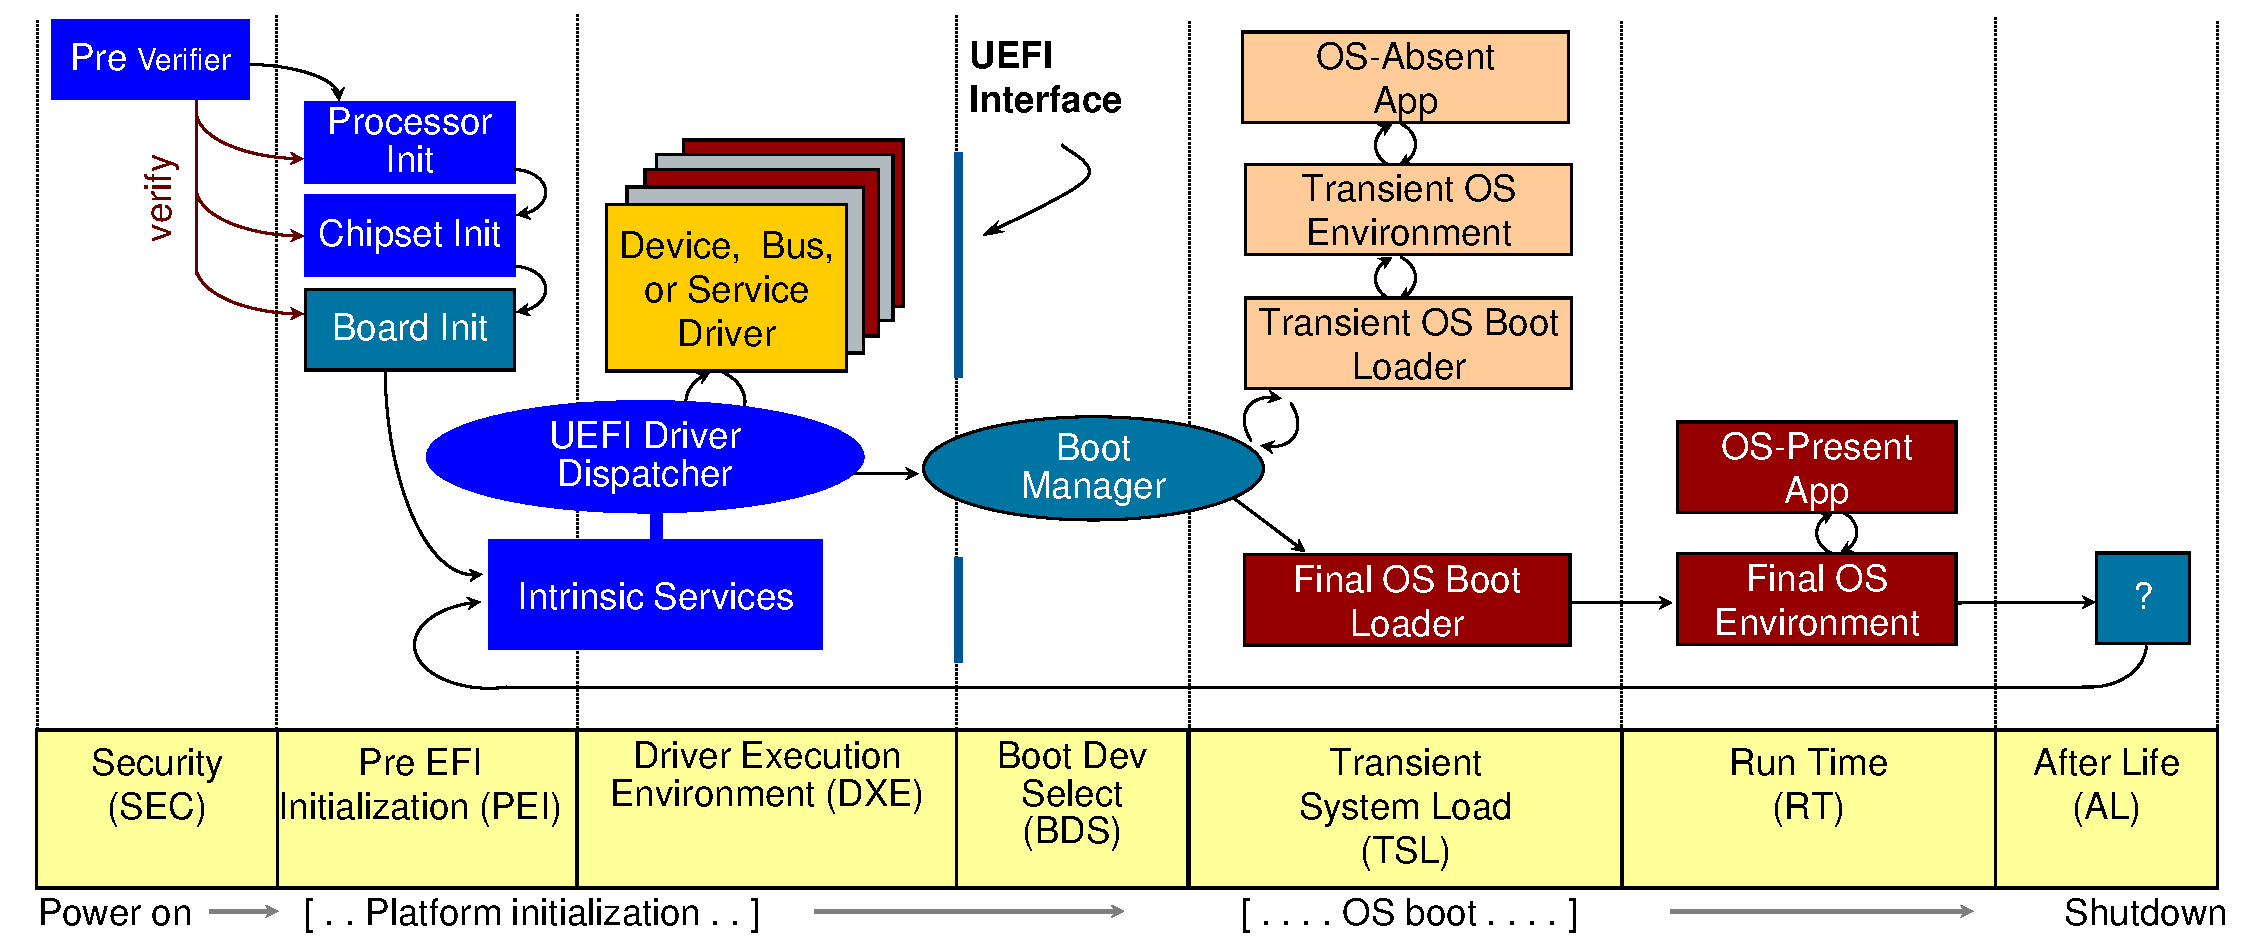
\includegraphics[width=\linewidth]{figure/mixed-figures/boot.pdf}
    \caption{UEFI启动过程}
    \label{fig:enter-label}
\end{figure}

这些固件代码段还会收集硬件信息,并且移交给操作系统。
早年的黑苹果、伪造OEM激活Windows 7都采用劫持UEFI启动后ACPI Table内容实现欺骗OS的效果。
在这个专题的实践中,我们需要体验读取、修改系统启动过程中的各个表,并且尝试传递更多的信息给操作系统。

\section{Read ACPI Table}
目标:修改EDK2的UEFI组件,在其中增加函数:\texttt{PrintAllACPITables}。该函数不传入任何参数,要求打印每一张表的地址、长度以及每一张其中所有的信息与校验信息。

可以参考EDK2下的\texttt{AcpiView},但是不得直接复制。

你也可以参考 EDK2 下的\texttt{Acpi.c} 中的 \texttt{EfiLocateFirstAcpiTable} 函数。

此外,关于 ACPI 的更多信息,可以参考\href{https://uefi.org/sites/default/files/resources/ACPI_Spec_6.5a_Final.pdf}{这本手册}来学习。

具体测评指标:
\begin{itemize}
\item 输出所有ACPI表的完整地址映射;
\item 每个表的输出必须包含:物理地址(64位十六进制)、表长度(32位十进制)、OEM ID(6字节ASCII)、校验和(8位十六进制)。
\end{itemize}

\section{Hack ACPI Table}
目标:修改EDK2的UEFI组件,在其中增加函数:\texttt{ChangeACPITable}。该函数传入一个\texttt{UINTN}的对象表明修改第几张表、输入\texttt{EFI\_ACPI\_DESCRIPTION\_HEADER*}表明待修改的数值,要求修改完成后打印每一张表的地址、长度以及每一张其中所有的信息与校验信息。

测试:通过引导Linux后读取对应的ACPI表检查输出进行验证。

具体评测指标:
\begin{itemize}
\item 修改\texttt{EFI\_ACPI\_DESCRIPTION\_HEADER}中所有字段(包括Signature保留字段)且自动生成正确校验和的比例达到100\%;
\item 系统重启3次后修改仍然有效;
\item 内核日志(\texttt{dmesg | grep ACPI})无CHECKSUM\_ERROR警告或其他ACPI警告。
\end{itemize}

\section{UEFI运行时服务}
目标:增加一个新的UEFI运行时服务,使得Linux系统可以调用这个新的服务导出硬件运行时信息。

提示:需要修改UEFI固件和Linux内核(sysfs部分),方便直接读取导出的结果。

测试:展示

\chapter{特权态与系统调用}
操作系统对特权态的管理是操作系统的重要组成部分,影响了用户态程序的编写。
这些系统调用也是操作系统向用户态提供抽象的重要部分,例如Linux中将设备的读写都转换为文件读写,因此对应的系统调用都和文件的操作读写相关。Windows的系统调用接口则更为复杂一些,因为其内核的构成并不是单纯的宏内核,对于最小执行单元也有不同的定义。
在这个专题的实践中,我们的目标是体验操作系统内核在通过系统调用进行系统管理上的重要作用。


\section{用户定义的系统调用}
目标:新增内核的键值存储模块(Key-Value Store),要求提供read接口和write接口。内核的键值数据需要存储在进程相关的结构体中,键值存储的对象是进程为对象。

提示:修改用户态系统调用的二进制文件和内核的系统调用接收器。

\subsection*{指标与评测要求}
\begin{itemize}
    \item 可评测指标:系统调用延迟(用户态到内核态切换时间+处理时间)、多线程下键值读写正确性(100并发线程下无竞争条件)
    \item 吞吐要求:单核每秒可处理不少于10,000次空操作读写请求
\end{itemize}

\subsection*{实现规范}
\begin{enumerate}
    \item 接口定义:
    \begin{lstlisting}[language=C]
    // 用户态接口
    int write_kv(int k, int v); // 返回写入字节数,错误返回-1
    int read_kv(int k);         // 成功返回对应值,错误返回-1
    \end{lstlisting}
    
    \item 内核侧实现:
    \begin{itemize}
        \item 在进程控制块(task\_struct)中添加kv\_store字段:\texttt{struct hlist\_head kv\_store[1024];}
        \item 采用开放寻址哈希表实现,哈希函数:\texttt{k \% 1024}
        \item 同步机制:每个哈希桶使用独立自旋锁(\texttt{spinlock\_t})
    \end{itemize}
    
\end{enumerate}

\subsection*{测试方案}
\begin{itemize}
    \item 创建100线程交替随机读写,最终验证数据一致性
    \item 使用sysbench工具发起100万次随机请求
    \item 开启KASAN和LOCKDEP内核调试选项下测试并发正确性
\end{itemize}

\section{vDSO}
在上一个体验中,你已经增加了系统调用感受到了系统的服务。然而每次系统调用还是需要通过异常或者中断进行特权态切换,会带来较大切换开销。
经过观察,可以发现一部分系统调用并不会泄露内核的状态也不会修改内核。
对于这些系统调用可以在用户态以只读共享页面的方式直接进行而无需进入操作系统内核。
Linux中提供了vDSO支持这一想法。

目标:在vDSO中新增一个读取当前进程对应的\texttt{task\_struct}中的所有信息的函数。

\subsection*{指标与评测要求}
\begin{itemize}
    \item 性能:读取数据延迟需小于100ns(依据机器有所不同)
    \item 正确性:返回的task\_struct指针地址与内核地址空间数据匹配
\end{itemize}

\subsection*{实现规范}
\begin{enumerate}
    \item 接口设计:
    \begin{lstlisting}[language=C]
    // vDSO暴露接口
    struct task_info {
        pid_t pid;
        void *task_struct_ptr;
        // 其他关键字段...
    };
    int get_task_struct_info(struct task_info *info);
    \end{lstlisting}
    
    \item 内核侧实现:
    \begin{itemize}
        \item 在vDSO镜像(arch/x86/entry/vdso/vdso.lds.S)添加新符号\_\_vdso\_get\_task\_info
        \item 实现函数填充current宏指向的task\_struct信息
        \item 用户态访问约束:所有指针字段标记为\texttt{\_\_user}属性
    \end{itemize}

\end{enumerate}

\subsection*{测试方案}
\begin{itemize}
    \item 对比从/proc/self/stat获取的pid与vDSO返回值
    \item 测试多次调用fork()的接口检查稳定性
\end{itemize}

\section{无需中断的系统调用}
通过vDSO,我们可以实现无需特权态切换对只读数据的访问。
那么对于需要请求内核服务的系统调用,是否也可以避开特权态切换呢?
答案是肯定的,FlexSC~\cite{soares2010flexsc}给出了对应的解决方案。
这一解决方案可以简化为用户态程序和操作系统内核存在共享页面,用户态程序将系统调用需要的参数写进这个共享页面,然后操作系统内核从这个共享页面中读取数据并且将结果写回该页面实现基于共享内存的系统调用。

目标:在Linux内核中实现无特权态切换的系统调用服务。

提示:用户态线程比较容易实现请求后等待结果的自旋,需要确保内核处理的线程始终在线。

\subsection*{指标与评测要求}
\begin{itemize}
    \item 吞吐和延迟要求:性能应当可以提升至少20\%。
    \item 兼容性:需通过Linux Test Project (LTP)全部系统调用相关测试用例
\end{itemize}


\subsection*{测试方案}
\begin{itemize}
    \item 吞吐:使用Apache Bench进行百万次getpid()调用测试
    \item 正确性:运行所有syscall/目录下的LTP测试用例
\end{itemize}

\chapter{内存管理}
在计算机系统(1)中,我们在虚拟存储器部分引出了交换空间的概念。管理内存是硬件和软件协同的结果。
在CPU启动后,内存的地址空间完整提供给第一个启动的软件,也就是操作系统。
随后操作系统在创建每一个进程时分配页表进行页映射,从而提供每个进程完整虚拟地址空间的抽象。
在这个专题的实践中,我们的目标是体验操作系统中不同的内存类型和对应管理内存的方式。

\section{页表和文件页}
目标:读取页表,并且手动修改页表页的映射实现共享(通过\texttt{mmap}调整映射,通过修改内核读取页表);设置文件页实现读写落在文件的指定区域中。

测试:测试页表映射和修改是否生效到文件中。

\section{内存文件系统}
Linux中提供了内存文件系统(RAMfs)的支持,其有MMU版本和NoMMU版本,分别位于\texttt{fs/ramfs/file-mmu.c}和\texttt{fs/ramfs/file-nommu.c}。
RAMfs无法持久化,在系统崩溃时文件会全部丢失。
现在你需要为RAMfs提供简单的持久化支持,当某个文件被flush到RAMfs时,该文件同步刷到一个预先设置的同步目录中以持久化该文件。

目标:增加flush下的文件持久化。

测试:测试持久化的文件内容语义和多线程持久化。



\section{内存压力导向的内存管理}
MacOS给出内存压力的概念,相比于UNIX的swap大小,它被认为是更好的表达虚拟内存健康程度的标志。

\begin{figure}[h]
    \centering
    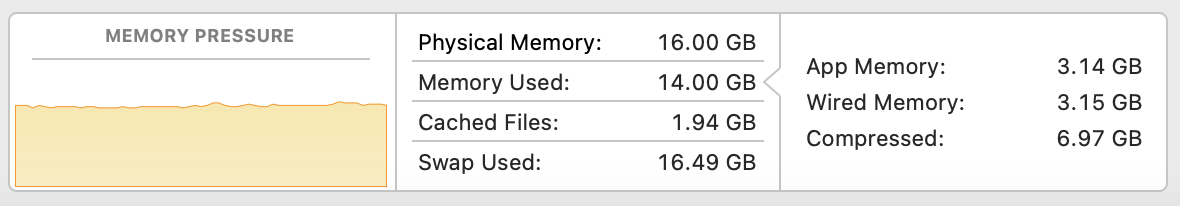
\includegraphics[width=0.8\linewidth]{figure/mixed-figures/memory-pressure.png}
    \caption{MacOS中的内存压力}
    \label{fig:enter-label}
\end{figure}

目标:该实践任务包含两个子任务点。
\begin{enumerate}
    \item 利用Linux的Wired Memory(即Active Memory)和压缩内存给出一个Linux下的内核内存压力指示器。
    \item 在用户态划出一块内存空间,实现一个简单的基于内存压力的交换策略。
\end{enumerate}


提示:区分wired memory和inactive memory的区别。

测试:测试内存压力和感知准确度的对比(演示),测试交换策略。

\chapter{文件系统}
文件是UNIX设计哲学中的一个重要组成部分,
一切皆文件的抽象使得用户调整系统的参数也变得更加简单。
因此,如何实现一个既能管理系统又能管理日常文件的文件系统便显得更加重要。
Linux通过一套统一的VFS(虚拟文件系统)抽象达成这一目标。
在本实践部分,你需要对VFS进行修改并且尝试使用文件系统。

\section{inode和扩展属性管理}

目标:读取设置inode的基本信息,引入新的\textbf{文件扩展属性(Extended file attributes)}。

测试:文件扩展属性的读写。



\section{用户态文件系统}
由于文件系统在Linux中被编译为内核对象(kernel object),文件系统崩溃会传导到内核造成内核不可用。此外,内核对象的灵活性较差。
Linux给出了FUSE的服务,允许在用户态实现一个文件系统。

目标:使用FUSE实现GPT服务。声明一个GPTfs,其中的目录为每一个对话session,对话session文件夹下的input为本轮用户输入的prompt,output文件为GPT输出的结果。每一轮对话都是单轮对话,无需考虑记录上下文。

测试:基本的读写效果

\section{用户空间下的内存磁盘}
随着硬件的发展,内存的价格已经显著下降。
内存的访问速度非常快,可以作为一部分反复读写的文件的临时存储。
在这一个任务中,你需要从用户态划出一块区域用于磁盘存储。

目标:使用FUSE实现RAMfs功能,要求读写碎片尽可能少并且支持硬链接。

提示:可以参考内核中RAMfs的功能,但是不要抄袭。

测试:文件读写和并发读写。

\chapter{网络与外部设备}
\section{tcpdump和socket管理}
Linux内核中提供了抓包等服务作为内核的网络套件的一部分。

目标:实现如下内容
\begin{enumerate}
    \item 按照一定条件进行抓包(要求修改tcpdump,不允许直接用现成的参数)
    \item 内核管理socket的安全性实现per-thread的socket fairness管理。
\end{enumerate}

测试:多Socket读写的管理(测试p99延迟)

\section{高速通信库:NCCL}
现代的高性能计算已经不能由单节点计算满足,需要多个节点多台机器进行并行计算。随着单节点算力的不断上升,并行计算时的通信成为了影响整个计算集群效率的关键因素。
传统的网络通信已经不能满足这一通信需求,各个计算卡的厂商普遍提供了自己的高速互联协议(如英伟达的NCCL、华为的HCCL)。
在这里给出一份可以用于学习参考的文档:\href{https://docs.nvidia.com/deeplearning/nccl/user-guide/docs/examples.html#communicator-creation-and-destruction-examples}{Nvidia NCCL examples}.
此外,源代码仓库为:\href{https://github.com/NVIDIA/nccl}{Nvidia NCCL}.

目标:通过NCCL实现简单的信息传输,比较和传统使用以太网的速度、正确性差异。



\section{数据平面开发套件:DPDK}
当前的网络协议都在内核空间中,因此涉及网络的操作都需要通过特权切换进入内核。
对于需要高速通信的程序,反复的上下文切换显然不符合要求。
不过,由于完整实现基于DPDK的通信所需要的代码量太大,我们在这里进行简化,只需要实现简单的网络即可。

目标:实现用户态基于DPDK的网络QoS管理,实现多个进程访问网络的带宽平衡。
% \chapter{安全与虚拟化}
% \section{常见的溢出攻击和侧信道攻击}

% \section{虚拟机调用Hypercall}

% \section{虚拟机内存访问加速}
\chapter{综合应用}
当你来到这一章节时,你应该对Linux内核的主要组成部分有了清晰的了解,对每个部分的修改效果应该也熟悉了。
在这个基础上,我们进一步探讨我们的综合应用。

\section{使用RDMA的远程内存Swap}
在这个项目中,你需要实现一个简单的使用远程内存的交换分区(swap)。具体而言,当缺页异常发生时,你需要使用RDMA访问远程内存将页面换到本地。如果远程页面不存在,你需要寻找本地交换文件中寻找这个目标页面。在两者都不存在的情况下,应当给出一个内存错误(如同访问非法地址的错误)。
\subsection{指标}
\paragraph*{项目形态。}
你的项目最终的形态应当符合以下指标:
\begin{enumerate}
    \item 将交换分区的内存页面通过RDMA存储到远程内存上。
    \item 设定一个可调整的比例决定远程内存和本地内存的比例。
    \item 对应用无感。
\end{enumerate}

\paragraph*{基础评测指标。}
项目的基础评测指标如下:
\begin{enumerate}
    \item 使用\texttt{memcached}~\cite{fitzpatrick2004distributed}存储一系列数据(YCSB~\cite{cooper2010benchmarking})在使用50\%远程内存时在50\%能够产生一个显著的时间差。
    \item 使用RDMA的交换时间需要比磁盘交换更短。
\end{enumerate}

对于基础评测指标,一个简单的示意图如图~\ref{fig:mixed:rdma-examples}所示。

\begin{figure}[h]
\centering
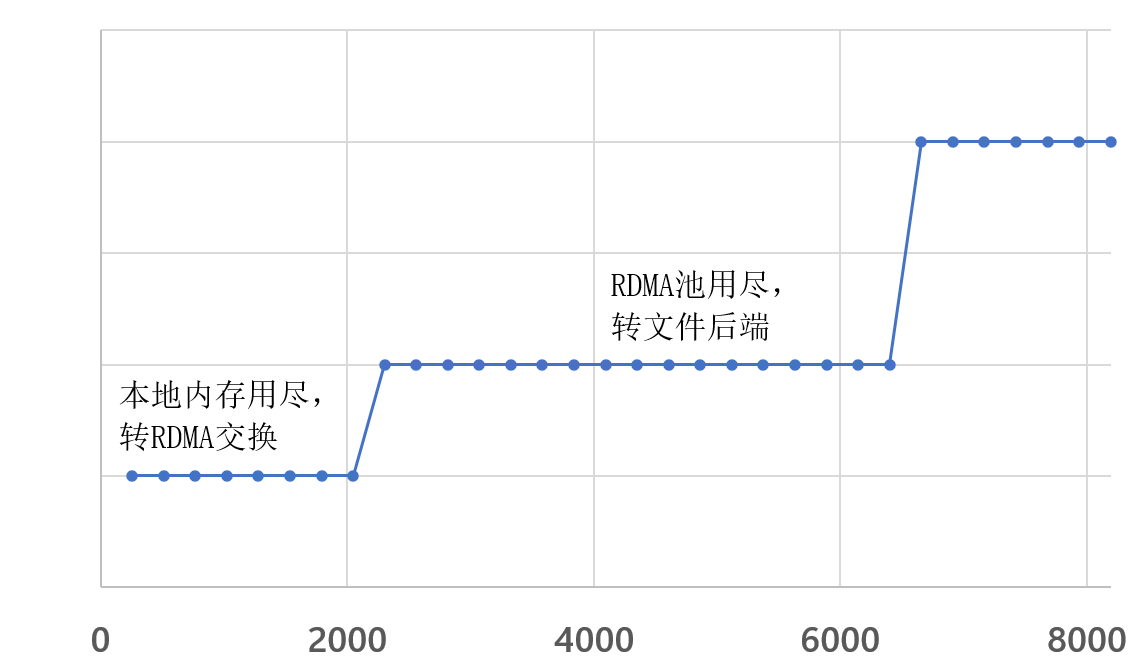
\includegraphics[scale=0.5]{figure/mixed-figures/RDMA-example.png}
\caption{RDMA和文件混合交换分区下的内存访问量同时间的示意图。图中假设本地内存为2048MB,RDMA内存约4096MB。相对时间仅为示意图,不代表真实场景数据。}
\label{fig:mixed:rdma-examples}
\end{figure}

\paragraph*{进阶指标。}
在基础评测的指标上,结合内存访问的特点,实现页预取和交换,目标发生尽可能少的缺页异常。

\subsection{快速上手和实现重点提示}
本项目的核心包括两个部分,内存管理和RDMA的访问。对于内存管理部分,需要修改原有系统的Page Fault处理流程。RDMA部分则需要维护RDMA连接确保发生缺页异常时向远端设备发起RDMA读写请求。

\paragraph*{内存管理。} 缺页异常发生后,操作系统需要确认这个页位于什么地方(是在内存中但是页表没有映射?还是这个页已经被交换到磁盘设备?或是这个页根本不存在?)。传统的顺序流程可以在体系结构下的\texttt{mm/fault.c}中找到相关的代码。加入RDMA后,需要保证RDMA部分不能被换出,并且加入对RDMA内存的搜索。

\paragraph*{RDMA管理。} RDMA的通信与不同的以太网通信不同。为了保证传输的速度,RDMA没有使用套接字(Socket)抽象。取而代之的是两大类Verbs(Memory Verbs和Message Verbs)这两大类的Verbs具体包含:Read(远程主机读取部分内存)、Write(数据写到远端主机)、Atomic(原子操作);Send(把数据发送到远程 QP 的接收队列里)、Receive(接收主机被告知接收到数据缓冲)。具体的管理可以参考以下链接:(中文)\url{https://zhuanlan.zhihu.com/p/649468433}(英语官方原版)\url{https://academy.nvidia.com/en/course/rdma-programming-intro/?cm=446}

\paragraph*{特殊点提示。}
\begin{itemize}
    \item 多线程的访问安全性:多个进程同时发生缺页异常在远端的处理过程;
    \item RDMA内存的管理:减少远端内存中的内存碎片。
\end{itemize}

\section{用户程序嵌入内核执行}
用户程序执行时需要通过系统调用(syscall)调用特权系统服务,每一次系统调用都有上下文切换的开销,从而使得密集调用系统调用的程序产生额外的开销。
一种简单的优化方法是将含有系统调用的程序嵌入内核执行,从而避免上下文切换。
这一更改实际上给内核打了很多的“洞”,忽略了内核的权限隔离,因此是不安全的。
我们深入之后会发现,这一想法的核心其实是一部分上下文权限隔离对程序而言过强了,程序没有用到对应的功能因此也不需要对应的隔离。
在这个基础上,我们可以通过为一些简单程序设计内核中隔离他们程序的方案。
具体而言,通过修改fork的过程将程序直接嵌入内核空间,增加一些特殊的机制(你自定义的机制,可以是页表、MPK等)实现该段代码在内核中仅能访问特定内存(相当于自己的地址空间)。
假设程序不是恶意的,因此不需要你考虑控制流完整性,但是需要注意代码的映射区域。
同时假设在这项作业中程序已经被编译为位置无关代码。


\subsection{指标}
\paragraph*{项目形态。}
你的项目最终的形态应当符合以下指标:
\begin{enumerate}
    \item 将一段程序嵌入到内核态执行,程序本身无需修改。
    \item 程序仅能访问自己的内存区间,而不能访问内核的其他数据结构。
\end{enumerate}

\paragraph*{基础评测指标。}
项目的基础评测指标如下:
\begin{enumerate}
    \item 一段仅包含一系列系统调用的程序可以进入内核实现吞吐的显著提升。
    \item 程序访问非法内存应当退出当前程序的执行,给出错误信息(可以在内核日志)并且不影响当前内核的执行。
    \item 支持多线程程序的执行,不影响多线程程序的可扩展性。
\end{enumerate}


\paragraph*{进阶指标。}
在基础评测的指标上,支持带有多个用户库文件的用户程序进入内核执行。

\subsection{快速上手和实现重点提示}
本项目的核心包括两个部分,代码启动阶段(fork)和执行阶段(exec)。

\paragraph*{启动阶段}
启动阶段用户程序并没有执行,核心需要考虑的部分是如何映射用户段的代码到内核空间,以及如何设置权限隔离的初始状态。
此外,需要在启动阶段拦截系统调用,确保系统调用转换为内核态的函数跳转。


\paragraph*{执行阶段}
执行阶段最核心的是在遇到错误的时候如何修正错误的状态,从而避免嵌入内核的程序崩溃内核。

\paragraph*{特殊点提示。}
\begin{itemize}
    \item 多线程执行:与内核线程的绑定执行关系;
    \item 内核状态的保护:防止单个程序崩溃整个内核。
\end{itemize}

\section{内核空间下的内存磁盘}
随着硬件的发展,内存的价格已经显著下降。
内存的访问速度非常快,可以作为一部分反复读写的文件的临时存储。
这一部分是用户空间下的内存磁盘的进一步延伸。


\subsection{指标}
\paragraph*{项目形态。}
你的项目最终的形态应当符合以下指标:
\begin{enumerate}
    \item 将一段内存空间作为磁盘空间映射给内核。
    \item 映射的磁盘空间可以进行文件读写和文件夹创建。
    \item 注册为一个磁盘设备而非文件系统。
\end{enumerate}

\paragraph*{基础评测指标。}
项目的基础评测指标如下:
\begin{enumerate}
    \item 使用\texttt{dd}一次性创建一个大文件的开销足够小(需要接近内存的读写速度)。
    \item 多次创建删除文件之后实际存储容量始终保持一致。
\end{enumerate}


\paragraph*{进阶指标。}
在基础评测的指标上,减小文件元数据的开销大小。

\subsection{快速上手和实现重点提示}
本项目的核心是内存空间的映射和分区管理。
与映射在用户空间不同,内核空间的映射需要保证用于虚拟磁盘的数据不能破坏内核数据的正确性。
此外,用户空间可以通过\texttt{fuse}实现用户态的分区访问。在内核中,该模块需要实现为内核模块,因此需要符合内核的一系列数据接口。

\paragraph*{特殊点提示。}
\begin{itemize}
    \item 多线程执行:多线程读写保证数据的一致性。
    \item 文件碎片:文件的碎片应该尽可能少。
\end{itemize}

\section{机密虚拟机Trapless的宿主协同内存管理}
机密虚拟机的一个核心是内存需要加密以防止宿主可以获取到虚拟机内存造成数据泄露,然而这样的安全措施也造成了宿主机无法感知虚拟机内的内存情况,内存分配无法最优化。
一种方式是虚拟机内核主动向宿主机的虚拟机管理器发起调用引导宿主机按照一定的偏好管理内存。
这种方式需要下陷到宿主机的虚拟机管理器,有较大的切换开销。
请设计一种机制,以不下陷的方式引导宿主机的按照一定偏好管理内存。



\subsection{指标}
\paragraph*{项目形态。}
你的项目最终的形态应当符合以下指标:
\begin{enumerate}
    \item 不修改虚拟机内应用程序,允许修改虚拟机管理器和虚拟机内的内核。
    \item 指示内存偏好时不发生下陷。
\end{enumerate}

\paragraph*{基础评测指标。}
项目的基础评测指标如下:
\begin{enumerate}
    \item 使用内存密集型任务在机密虚拟机内部设置特定内存位置后计算速度和用户态的读写速度一致。
\end{enumerate}


\subsection{快速上手和实现重点提示}
本项目的指标较少,因为核心代码需要较大的修改,包括三个部分:宿主机的内核、虚拟机的内核、宿主机的虚拟机管理器。
宿主机内核需要设定特殊的接口管理加密的内存页面。
虚拟机内核需要修改实现无下陷与宿主机的虚拟机管理器进行交互。
宿主机的虚拟机内存管理器需要增加接收虚拟机内核的特殊内存偏好参数并且传递给宿主机。

\paragraph*{特殊点提示。}
\begin{itemize}
    \item 虚拟机下陷的处理。
    \item 共享内存页的管理。
    \item 宿主机的内存管理。
\end{itemize}
% \chapter{Elegant\LaTeX{} 系列模板介绍}

% Elegant\LaTeX{} 项目组致力于打造一系列美观、优雅、简便的模板方便用户使用。目前由 \href{https://github.com/ElegantLaTeX/ElegantNote}{ElegantNote},\href{https://github.com/ElegantLaTeX/ElegantBook}{ElegantBook},\href{https://github.com/ElegantLaTeX/ElegantPaper}{ElegantPaper} 组成,分别用于排版笔记,书籍和工作论文。强烈推荐使用最新正式版本!本文将介绍本模板的一些设置内容以及基本使用方法。如果您有其他问题,建议或者意见,欢迎在 GitHub 上给我们提交 \href{https://github.com/ElegantLaTeX/ElegantBook/issues}{issues} 或者邮件联系我们。

% 我们的联系方式如下,建议加入用户 QQ 群提问,这样能更快获得准确的反馈,加群时请备注 \LaTeX{} 或者 Elegant\LaTeX{} 相关内容。
% \begin{itemize}
%   \item 官网:\href{https://elegantlatex.org/}{https://elegantlatex.org/}(暂时歇业)
%   \item GitHub 地址:\href{https://github.com/ElegantLaTeX/}{https://github.com/ElegantLaTeX/}
%   \item Gitee 地址:\href{https://gitee.com/ElegantLaTeX}{https://gitee.com/ElegantLaTeX}
%   \item CTAN 地址:\href{https://ctan.org/pkg/elegantbook}{https://ctan.org/pkg/elegantbook}
%   \item 下载地址:\href{https://github.com/ElegantLaTeX/ElegantBook/releases}{正式发行版},\href{https://github.com/ElegantLaTeX/ElegantBook/archive/master.zip}{最新版}
%   \item 微博:Elegant\LaTeX{}(密码有点忘了)
%   \item 微信公众号:Elegant\LaTeX{}(不定期更新)
%   \item 用户 QQ 群:692108391(建议加群)
%   \item 邮件:\email{elegantlatex2e@gmail.com}
% \end{itemize}

% \section{模板安装与更新}

% 你可以通过免安装的方式使用本模板,包括在线使用和本地(文件夹内)使用两种方式,也可以通过 \TeX{} 发行版安装使用。

% \subsection{在线使用模板}

% 我们把三套模板全部上传到 \href{https://www.overleaf.com/}{Overleaf} 上了,网络便利的用户可以直接通过 Overleaf 在线使用我们的模板。使用 Overleaf 的好处是无需安装 \TeX{} Live,可以随时随地访问自己的文件。查找模板,请在 Overleaf 模板库里面搜索 \lstinline{elegantlatex} 即可,你也可以直接访问\href{https://www.overleaf.com/latex/templates?addsearch=elegantlatex}{搜索结果}。选择适当的模板之后,将其 \lstinline{Open as Template},即可把模板存到自己账户下,然后可以自由编辑以及与别人一起协作。更多关于 Overleaf 的介绍和使用,请参考 Overleaf 的\href{https://www.overleaf.com/learn}{官方文档}。

% \subsection{本地免安装使用}

% \textbf{免安装}使用方法如下:从 GitHub 或者 CTAN 下载最新版,严格意义上只需要类文件 \lstinline{elegantbook.cls}。然后将模板文件放在你的工作目录下即可使用。这样使用的好处是,无需安装,简便;缺点是,当模板更新之后,你需要手动替换 \lstinline{cls} 文件。

% \subsection{发行版安装与更新}

% 本模板测试环境为 
% \begin{enumerate}
%   \item Win10 + \TeX{} Live 2022;
%   \item Ubuntu 20.04 + \TeX{} Live 2022;
%   \item macOS Monterey + Mac\TeX{} 2022。
% \end{enumerate}

% \TeX Live/Mac\TeX{} 的安装请参考啸行的\href{https://github.com/OsbertWang/install-latex-guide-zh-cn/releases/}{一份简短的关于安装 \LaTeX{} 安装的介绍}。

% 安装 \TeX{} Live 之后,安装后建议升级全部宏包,升级方法:使用 cmd 或 terminal 运行 \lstinline{tlmgr update --all},如果 tlmgr 需要更新,请使用 cmd 运行 \lstinline{tlmgr update --self},如果更新过程中出现了中断,请改用 \lstinline{tlmgr update --self --all --reinstall-forcibly-removed} 更新,也即

% \begin{lstlisting}
% tlmgr update --self 
% tlmgr update --all
% tlmgr update --self --all --reinstall-forcibly-removed
% \end{lstlisting}

% 更多的内容请参考 \href{https://tex.stackexchange.com/questions/55437/how-do-i-update-my-tex-distribution}{How do I update my \TeX{} distribution?}

% \subsection{其他发行版本}

% 由于宏包版本问题,本模板不支持 C\TeX{} 套装,请务必安装 TeX Live/Mac\TeX{}。更多关于 \TeX{} Live 的安装使用以及 C\TeX{} 与 \TeX{} Live 的兼容、系统路径问题,请参考官方文档以及啸行的\href{https://github.com/OsbertWang/install-latex-guide-zh-cn/releases/}{一份简短的关于安装 \LaTeX{} 安装的介绍}。


% \section{关于提交}

% 出于某些因素的考虑,Elegant\LaTeX{} 项目自 2019 年 5 月 20 日开始,\textbf{不再接受任何非作者预约性质的提交}(pull request)!如果你想改进模板,你可以给我们提交 issues,或者可以在遵循协议(LPPL-1.3c)的情况下,克隆到自己仓库下进行修改。


% \chapter{ElegantBook 设置说明}

% 本模板基于基础的 book 文类,所以 book 的选项对于本模板也是有效的(纸张无效,因为模板有设备选项)。默认编码为 UTF-8,推荐使用 \TeX{} Live 编译。

% \section{语言模式}
% 本模板内含两套基础语言环境 \lstinline{lang=cn}、\lstinline{lang=en}。改变语言环境会改变图表标题的引导词(图,表),文章结构词(比如目录,参考文献等),以及定理环境中的引导词(比如定理,引理等)。不同语言模式的启用如下:
% \begin{lstlisting}
% \documentclass[cn]{elegantbook} 
% \documentclass[lang=cn]{elegantbook}
% \end{lstlisting}

% 除模板自带的两套语言设定之外,由\textbf{网友}提供的其他语言环境设置如下:
% \begin{itemize}
%   \item 由 \href{https://github.com/VincentMVV}{VincentMVV} 提供的意大利语翻译 \lstinline{lang=it},相关讨论见 \href{https://github.com/ElegantLaTeX/ElegantBook/issues/85}{Italian translation};
%   \item 由 \href{https://github.com/abfek66}{abfek66} 提供的法语翻译 \lstinline{lang=fr},相关讨论见 \href{https://github.com/ElegantLaTeX/ElegantBook/issues/85}{Italian translation};
%   % \item 由 \href{https://github.com/stultus}{stultus} 提供的马拉雅拉姆语翻译 \lstinline{lang=},相关讨论见 \href{https://github.com/ElegantLaTeX/ElegantBook/issues/90}{Malayalam translation};
%   \item 由 \href{https://github.com/inktvis75}{inktvis75} 提供的荷兰语翻译 \lstinline{lang=nl},相关讨论见 \href{https://github.com/ElegantLaTeX/ElegantBook/issues/108}{Dutch Translation};
%   \item 由 \href{https://github.com/palkotamas}{palkotamas} 提供的匈牙利语翻译 \lstinline{lang=hu},相关讨论见 \href{https://github.com/ElegantLaTeX/ElegantBook/issues/111}{Hungarian translation};
%   \item 由 Lisa 提供的德语翻译 \lstinline{lang=de},相关讨论见 \href{https://github.com/ElegantLaTeX/ElegantBook/issues/113}{Deutsch translation};
%   \item 由 Gustavo A. Corradi 提供的西班牙语的翻译 \lstinline{lang=es},相关讨论见 \href{https://github.com/ElegantLaTeX/ElegantBook/issues/133}{Spanish translation};
%   \item 由 \href{https://github.com/Altantsooj}{Altantsooj} 提供的蒙古语的翻译 \lstinline{lang=mn},相关讨论见 \href{https://github.com/ElegantLaTeX/ElegantBook/issues/137}{Mongolian translation};
%   \item 由 \href{https://github.com/inusturbo}{inusturbo} 提供的日本语的翻译 \lstinline{lang=jp},相关讨论见 \href{https://github.com/ElegantLaTeX/ElegantBook/issues/172}{Japanese Translation}。
% \end{itemize}



% \begin{remark}
% 以上各个语言的设定均为网友设定,我们未对上述翻译进行过校对,如果有问题,请在对应的 issue 下评论。并且,只有中文环境(\lstinline{lang=cn})才可以输入中文。
% \end{remark}

% \section{设备选项}
% 最早我们在 ElegantNote 模板中加入了设备选项(\lstinline{device}),后来,我们觉得这个设备选项的设置可以应用到 ElegantBook 中\footnote{不过因为 ElegantBook 模板封面图片的存在,在修改页面设计时,需要对图片进行裁剪。},而且 Book 一般内容比较多,如果在 iPad 上看无需切边,放大,那用户的阅读体验将会得到巨大提升。你可以使用下面的选项将版面设置为 iPad 设备模式\footnote{默认为 normal 模式,也即 A4 纸张大小。}
% \begin{lstlisting}
% \documentclass[pad]{elegantbook} %or
% \documentclass[device=pad]{elegantbook}
% \end{lstlisting}

% \section{颜色主题}

% 本模板内置 5 组颜色主题,分别为 \textcolor{structure1}{\lstinline{green}}\footnote{为原先默认主题。}、\textcolor{structure2}{\lstinline{cyan}}、\textcolor{structure3}{\lstinline{blue}}(默认)、\textcolor{structure4}{\lstinline{gray}}、\textcolor{structure5}{\lstinline{black}}。另外还有一个自定义的选项  \lstinline{nocolor}。调用颜色主题 \lstinline{green} 的方法为 
% \begin{lstlisting}
% \documentclass[green]{elegantbook} %or
% \documentclass[color=green]{elegantbook}
% \end{lstlisting}


% \begin{table}[htbp]
%   \caption{ElegantBook 模板中的颜色主题\label{tab:color thm}}
%   \centering
%   \begin{tabular}{ccccccc}
%   \toprule
%     & \textcolor{structure1}{green} 
%     & \textcolor{structure2}{cyan} 
%     & \textcolor{structure3}{blue}
%     & \textcolor{structure4}{gray} 
%     & \textcolor{structure5}{black} 
%     & 主要使用的环境\\
%   \midrule
%     structure & \ccr{structure1}
%     & \ccr{structure2}
%     & \ccr{structure3} 
%     & \ccr{structure4} 
%     & \ccr{structure5} 
%     & chapter \ section \ subsection \\
%     main      & \ccr{main1}
%     & \ccr{main2}
%     & \ccr{main3}
%     & \ccr{main4}
%     & \ccr{main5}
%     & definition \ exercise \ problem \\
%     second    & \ccr{second1}
%     & \ccr{second2}
%     & \ccr{second3}
%     & \ccr{second4}
%     & \ccr{second5}
%     & theorem \ lemma \ corollary\\
%     third     & \ccr{third1}
%     & \ccr{third2}
%     & \ccr{third3}
%     & \ccr{third4}
%     & \ccr{third5}
%     & proposition\\
%   \bottomrule
%   \end{tabular}
% \end{table}

% 如果需要自定义颜色的话请选择 \lstinline{nocolor} 选项或者使用 \lstinline{color=none},然后在导言区定义 structurecolor、main、second、third 颜色,具体方法如下:
% \begin{lstlisting}[tabsize=4]
% \definecolor{structurecolor}{RGB}{0,0,0}
% \definecolor{main}{RGB}{70,70,70}    
% \definecolor{second}{RGB}{115,45,2}    
% \definecolor{third}{RGB}{0,80,80}
% \end{lstlisting}

% \section{封面}

% \subsection{封面个性化}

% 从 3.10 版本开始,封面更加弹性化,用户可以自行选择输出的内容,包括 \lstinline{\title} 在内的所有封面元素都可为空。目前封面的元素有

% \begin{table}[htbp]
%   \centering
%   \caption{封面元素信息}
%   \begin{tabular}{p{0.07\textwidth}p{0.15\textwidth}|p{0.07\textwidth}p{0.15\textwidth}|p{0.07\textwidth}p{0.15\textwidth}}
%     \toprule
%     信息 & 命令 & 信息 & 命令 & 信息 & 命令 \\
%     \midrule
%     标题 & \lstinline|\title| & 副标题 & \lstinline|\subtitle| & 作者 & \lstinline|\author| \\
%     机构 & \lstinline|\institute| & 日期 &  \lstinline|\date| & 版本 & \lstinline|\version| \\
%     箴言 & \lstinline|\extrainfo| & 封面图 & \lstinline|\cover| & 徽标 & \lstinline|\logo| \\
%     \bottomrule
%   \end{tabular}
% \end{table}

% 另外,额外增加一个 \lstinline{\bioinfo} 命令,有两个选项,分别是信息标题以及信息内容。比如需要显示{\kaishu User Name:111520},则可以使用 
% \begin{lstlisting}
% \bioinfo{User Name}{115520}
% \end{lstlisting}

% 封面中间位置的色块的颜色可以使用下面命令进行修改:
% \begin{lstlisting}
% \definecolor{customcolor}{RGB}{32,178,170}
% \colorlet{coverlinecolor}{customcolor}
% \end{lstlisting}

% \subsection{封面图}

% 本模板使用的封面图片来源于 \href{https://pixabay.com/en/tea-time-poetry-coffee-reading-3240766/}{pixabay.com}\footnote{感谢 China\TeX{} 提供免费图源网站,另外还推荐 \href{https://www.pexels.com/}{pexels.com}。},图片完全免费,可用于任何场景。封面图片的尺寸为 $1280 \times 1024$, 更换图片的时候请\textbf{严格}按照封面图片尺寸进行裁剪。推荐一个免费的在线图片裁剪网站 \href{https://www.fotor.com/cn}{fotor.com}。用户 QQ 群内有一些合适尺寸的封面,欢迎取用。

% \subsection{徽标}

% 本文用到的 Logo 比例为 1:1,也即正方形图片,在更换图片的时候请选择合适的图片进行替换。

% \subsection{自定义封面}

% 另外,如果使用自定义的封面,比如 Adobe illustrator 或者其他软件制作的 A4 PDF 文档,请把 \lstinline{\maketitle} 注释掉,然后借助 \lstinline{pdfpages} 宏包将自制封面插入即可。如果使用 \lstinline{titlepage} 环境,也是类似。如果需要 2.x 版本的封面,请参考 \href{https://github.com/EthanDeng/etitlepage}{etitlepage}。

% \section{章标标题}

% 本模板内置 2 套\textit{章标题显示风格},包含 \lstinline{hang}(默认)与 \lstinline{display} 两种风格,区别在于章标题单行显示(\lstinline{hang})与双行显示(\lstinline{display}),本说明使用了 \lstinline{hang}。调用方式为
% \begin{lstlisting}
% \documentclass[hang]{elegantbook} %or
% \documentclass[titlestyle=hang]{elegantbook}
% \end{lstlisting}

% 在章标题内,章节编号默认是以数字显示,也即{\kaishu 第 1 章},{\kaishu 第 2 章}等等,如果想要把数字改为中文,可以使用
% \begin{lstlisting}
% \documentclass[chinese]{elegantbook} %or
% \documentclass[scheme=chinese]{elegantbook}
% \end{lstlisting}

% \section{数学环境简介}

% 在我们这个模板中,我们定义了两种不同的定理模式 \lstinline{mode},包括简单模式(\lstinline{simple})和炫彩模式(\lstinline{fancy}),默认为 \lstinline{fancy} 模式,不同模式的选择为
% \begin{lstlisting}
% \documentclass[simple]{elegantbook} %or
% \documentclass[mode=simple]{elegantbook}
% \end{lstlisting}

% 本模板定义了四大类环境

% \begin{itemize}
%   \item \textit{定理类环境},包含标题和内容两部分,全部定理类环境的编号均以章节编号。根据格式的不同分为 3 种
%     \begin{itemize}
%       \item \textcolor{main}{\textbf{definition}} 环境,颜色为 \textcolor{main}{main};
%       \item \textcolor{second}{\textbf{theorem、lemma、corollary、axiom、postulate}} 环境,颜色为 \textcolor{second} {second};
%       \item \textcolor{third}{\textbf{proposition}} 环境,颜色为 \textcolor{third}{third}。
%     \end{itemize}
%   \item \textit{示例类环境},有 \textbf{example、problem、exercise} 环境(对应于例、例题、练习),自动编号,编号以章节为单位,其中 \textbf{exercise} 有提示符。
%   \item \textit{提示类环境},有 \textbf{note} 环境,特点是:无编号,有引导符。
%   \item \textit{结论类环境},有 \textbf{conclusion、assumption、property、remark、solution} 环境\footnote{本模板还添加了一个 result 选项,用于隐藏 \lstinline{solution} 和 \lstinline{proof} 环境,默认为显示(\lstinline{result=answer}),隐藏使用 \lstinline{result=noanswer}。},三者均以粗体的引导词为开头,和普通段落格式一致。
% \end{itemize}

% \subsection{定理类环境的使用}

% 由于本模板使用了 \lstinline{tcolorbox} 宏包来定制定理类环境,所以和普通的定理环境的使用有些许区别,定理的使用方法如下:
% \begin{lstlisting}
% \begin{theorem}{theorem name}{label}
%   The content of theorem.
% \end{theorem}
% \end{lstlisting}

% 第一个必选项 \lstinline{theorem name} 是定理的名字,第二个必选项 \lstinline{label} 是交叉引用时所用到的标签,交叉引用的方法为 \verb|\ref{thm:label}|。请注意,交叉引用时必须加上前缀 \lstinline{thm:}。

% 在用户多次反馈下,4.x 之后,引入了原生定理的支持方式,也就是使用可选项方式:

% \begin{lstlisting}
% \begin{theorem}[theorem name] \label{thm:theorem-label}
%   The content of theorem.
% \end{theorem}
% % or 
% \begin{theorem} \label{thm:theorem-withou-name}
%   The content of theorem without name.
% \end{theorem}
% \end{lstlisting}

% 其他相同用法的定理类环境有:

% \begin{table}[htbp]
%    \centering
%    \caption{定理类环境}
%      \begin{tabular}{llll}
%      \toprule
%      环境名 & 标签名 & 前缀 & 交叉引用 \\
%      \midrule
%      definition & label & def   & \lstinline|\ref{def:label}| \\
%      theorem & label & thm   & \lstinline|\ref{thm:label}| \\
%      postulate & label & pos & \lstinline|\ref{pos:label}| \\
%      axiom & label & axi & \lstinline|\ref{axi:label}|\\
%      lemma & label & lem   & \lstinline|\ref{lem:label}| \\
%      corollary & label & cor   & \lstinline|\ref{cor:label}| \\
%      proposition & label & pro   & \lstinline|\ref{pro:label}| \\
%      \bottomrule
%      \end{tabular}%
%    \label{tab:theorem-class}%
%  \end{table}%
 
% % \subsection{算法环境}

 
% % \begin{algorithm}\label{alg:test}
% %   \Input{A bitmap $I$ of size $w \times l$}
% %   \Output{A partition of the bitmap}
% %   \BlankLine
% %   \emph{special treatment of the first line}\;
% %   \For{$i \leftarrow 2$ \KwTo $l$}{
% %     \emph{special treatment of the first element of line $i$}\;
% %     \For{$j \leftarrow 2$ \KwTo $w$}{\label{forins}
% %       $\Left \leftarrow \FindCompress{$I[i,j-1]$}$\;
% %       $\Up \leftarrow \FindCompress{$I[i-1,]$}$\;
% %       $\This \leftarrow \FindCompress{$I[i,j]$}$\;
% %       \If(\tcp*[h]{O(\Left,\This)==1}){\Left compatible with \This}{\label{lt}
% %         \lIf{$\Left < \This$}{$\Union{\Left,\This}$}
% %         \lElse{$\Union{\This,\Left}$}
% %       }
% %       \If(\tcp*[f]{O(\Up,\This)==1}){\Up compatible with \This}{\label{ut}
% %         \lIf{$\Up < \This$}{$\Union{\Up,\This}$}
% %         \tcp{\This is put under \Up to keep tree as flat as possible}\label{cmt}
% %         \lElse{$\Union{\This,\Up}$}\tcp*[r]{\This{} linked to \Up}\label{lelse}
% %       }
% %     }
% %     \lForEach{element $e$ of the line $i$}{\FindCompress{p}}
% %   }
% %   \caption{disjoint decomposition}\label{algo_disjdecomp}
% % \end{algorithm}


% \subsection{修改计数器}

% 当前定理等环境计数器按章计数,如果想修改定理类环境按节计数,可以修改计数器选项 thmcnt:

% \begin{lstlisting}
%   \documentclass[section]{elegantbook} %or
%   \documentclass[thmcnt=section]{elegantbook}
% \end{lstlisting}


% \subsection{其他环境的使用}

% 其他三种环境没有选项,可以直接使用,比如 \lstinline{example} 环境的使用方法与效果:
% \begin{lstlisting}
% \begin{example}
%    This is the content of example environment.
% \end{example}
% \end{lstlisting}

% 这几个都是同一类环境,区别在于

% \begin{itemize}
%   \item 示例环境(example)、练习(exercise)与例题(problem)章节自动编号;
%   \item 注意(note),练习(exercise)环境有提醒引导符;
%   \item 结论(conclusion)等环境都是普通段落环境,引导词加粗。
% \end{itemize}

% \section{列表环境}
% 本模板借助于 \lstinline{tikz} 定制了 \lstinline{itemize} 和 \lstinline{enumerate} 环境,其中 \lstinline{itemize} 环境修改了 3 层嵌套,而 \lstinline{enumerate} 环境修改了 4 层嵌套(仅改变颜色)。示例如下\\[2ex]
% \begin{minipage}[b]{0.49\textwidth}
%   \begin{itemize}
%     \item first item of nesti;
%     \item second item of nesti;
%       \begin{itemize}
%         \item first item of nestii;
%         \item second item of nestii;
%         \begin{itemize}
%           \item first item of nestiii;
%           \item second item of nestiii.
%         \end{itemize}   
%       \end{itemize}
%   \end{itemize}
% \end{minipage}
% \begin{minipage}[b]{0.49\textwidth}
%   \begin{enumerate}
%     \item first item of nesti;
%     \item second item of nesti;
%       \begin{enumerate}
%         \item first item of nestii;
%         \item second item of nestii;
%         \begin{enumerate}
%           \item first item of nestiii;
%           \item second item of nestiii.
%         \end{enumerate}   
%       \end{enumerate}
%   \end{enumerate}
% \end{minipage}

% \section{参考文献}
% 文献部分,本模板调用了 biblatex 宏包,并提供了 biber(默认) 和 bibtex 两个后端选项,可以使用 \lstinline{bibend} 进行修改:

% \begin{lstlisting}
%   \documentclass[bibtex]{elegantbook}
%   \documentclass[bibend=bibtex]{elegantbook}
% \end{lstlisting}

% 关于文献条目(bib item),你可以在谷歌学术,Mendeley,Endnote 中取,然后把它们添加到 \lstinline{reference.bib} 中。在文中引用的时候,引用它们的键值(bib key)即可。

% 为了方便文献样式修改,模板引入了 \lstinline{bibstyle} 和 \lstinline{citestyle} 选项,默认均为数字格式(numeric),参考文献示例:\cite{cn1,en2,en3} 使用了中国一个大型的 P2P 平台(人人贷)的数据来检验男性投资者和女性投资者在投资表现上是否有显著差异。

% 如果需要设置为国标 GB7714-2015,需要使用:
% \begin{lstlisting}
%   \documentclass[citestyle=gb7714-2015, bibstyle=gb7714-2015]{elegantbook} 
% \end{lstlisting}

% 如果需要添加排序方式,可以在导言区加入
% \begin{lstlisting}
%   \ExecuteBibliographyOptions{sorting=ynt}
% \end{lstlisting}

% 启用国标之后,可以加入 \lstinline{sorting=gb7714-2015}。

% \section{添加序章}

% 如果你想在第一章前面添序章,不改变原本章节序号,可以在第一章内容前面使用 
% \begin{lstlisting}
% \chapter*{Introduction}
% \markboth{Introduction}{Introduction}
% The content of introduction.
% \end{lstlisting}

% \section{目录选项与深度}
% 本模板添加了一个目录选项 \lstinline{toc},可以设置目录为单栏(\lstinline{onecol})和双栏(\lstinline{twocol})显示,比如双栏显示可以使用
% \begin{lstlisting}
% \documentclass[twocol]{elegantbook}
% \documentclass[toc=twocol]{elegantbook}
% \end{lstlisting}

% 默认本模板目录深度为 1,你可以在导言区使用
% \begin{lstlisting}
% \setcounter{tocdepth}{2}
% \end{lstlisting}
% 将其修改为 2 级目录(章与节)显示。


% \section{章节摘要}
% 模板新增了一个章节摘要环境(introduction),使用示例
% \begin{lstlisting}
% \begin{introduction}
%   \item Definition of Theorem
%   \item Ask for help
%   \item Optimization Problem
%   \item Property of Cauchy Series
%   \item Angle of Corner
% \end{introduction}
% \end{lstlisting}
% 效果如下:
% \begin{introduction}
%   \item Definition of Theorem
%   \item Ask for help
%   \item Optimization Problem
%   \item Property of Cauchy Series
%   \item Angle of Corner
% \end{introduction}

% 环境的标题文字可以通过这个环境的可选参数进行修改,修改方法为:
% \begin{lstlisting}
% \begin{introduction}[Brief Introduction]
% ...
% \end{introduction}
% \end{lstlisting}

% \section{章后习题}
% 前面我们介绍了例题和练习两个环境,这里我们再加一个,章后习题(\lstinline{problemset})环境,用于在每一章结尾,显示本章的练习。使用方法如下

% \begin{lstlisting}
% \begin{problemset}
%   \item exercise 1
%   \item exercise 2
%   \item exercise 3
% \end{problemset}
% \end{lstlisting}


% 效果如下:
% \begin{problemset}
%   \item exercise 1
%   \item exercise 2
%   \item exercise 3
%   \item 测试数学公式
%   \begin{equation}
%     a^2+b^2=c_{2_{i}} (1,2) [1,23]
%   \end{equation}
% \end{problemset}

% \begin{remark}
% 如果你想把 \lstinline{problemset} 环境的标题改为其他文字,你可以类似于 introduction 环境修改 problemset 的可选参数。另外,目前这个环境会自动出现在目录中,但是不会出现在页眉页脚信息中(待解决)。
% \end{remark}

% \begin{solution}
% 如果你想把 \lstinline{problemset} 环境的标题改为其他文字,你可以类似于 introduction 环境修改 problemset 的可选参数。另外,目前这个环境会自动出现在目录中,但是不会出现在页眉页脚信息中(待解决)。
% \end{solution}

% \section{旁注}

% 在 3.08 版本中,我们引入了 旁注设置选项 \lstinline{marginpar=margintrue} 以及测试命令 \lstinline{\elegantpar} ,但是由此带来一堆问题。我们决定在 3.09 版本中将其删除,并且,在旁注命令得到大幅度优化之前,不会将此命令再次引入书籍模板中。对此造成各位用户的不方便,非常抱歉!不过我们保留了 \lstinline{marginpar} 这个选项,你可以使用 \lstinline{marginpar=margintrue} 获得保留右侧旁注的版面设计。然后使用系统自带的 \lstinline{\marginpar} 或者 \lstinline{marginnote} 宏包的 \lstinline{\marginnote} 命令。

% \begin{remark}
% 在使用旁注的时候,需要注意的是,文本和公式可以直接在旁注中使用。

% \begin{lstlisting}
% % text
% \marginpar{margin paragraph text}

% % equation
% \marginpar{
%   \begin{equation}
%     a^2 + b^2 = c^2
%   \end{equation}
% }
% \end{lstlisting}

% 但是浮动体(表格、图片)需要注意,不能用浮动体环境,需要使用直接插图命令或者表格命令环境。然后使用 \lstinline{\captionof} 为其设置标题。为了得到居中的图表,可以使用 \lstinline{\centerline} 命令或者 \lstinline{center} 环境。更多详情请参考:\href{https://tex.stackexchange.com/questions/5583/caption-of-figure-in-marginpar-and-caption-of-wrapfigure-in-margin}{Caption of Figure in Marginpar}。

% \begin{lstlisting}
% % graph with centerline command
% \marginpar{
%   \centerline{
%     \includegraphics[width=0.2\textwidth]{logo.png}
%   }
%   \captionof{figure}{your figure caption}
% }

% % graph with center environment
% \marginpar{
%   \begin{center}
%     \includegraphics[width=0.2\textwidth]{logo.png}
%     \captionof{figure}{your figure caption}
%   \end{center}
% }
% \end{lstlisting}

% \end{remark}

% \chapter{字体选项}
% 字体选项独立成章的原因是,我们希望本模板的用户关心模板使用的字体,知晓自己使用的字体以及遇到字体相关的问题能更加便捷地找到答案。

% \textcolor{red}{\bfseries 重要提示}:从 3.10 版本更新之后,沿用至今的 newtx 系列字体被重新更改为 cm 字体。并且新增中文字体(\lstinline{chinesefont})选项。

% \section{数学字体选项}

% 本模板定义了一个数学字体选项(\lstinline{math}),可选项有三个:
% \begin{enumerate}
%   \item \lstinline{math=cm}(默认),使用 \LaTeX{} 默认数学字体(推荐,无需声明);
%   \item \lstinline{math=newtx},使用 \lstinline{newtxmath} 设置数学字体(潜在问题比较多)。
%   \item \lstinline{math=mtpro2},使用 \lstinline{mtpro2} 宏包设置数学字体,要求用户已经成功安装此宏包。
% \end{enumerate}

% \section{使用 newtx 系列字体}

% 如果需要使用原先版本的 \lstinline{newtx} 系列字体,可以通过显示声明数学字体:

% \begin{lstlisting}
% \documentclass[math=newtx]{elegantbook}
% \end{lstlisting}

% \subsection{连字符}

% 如果使用 \lstinline{newtx} 系列字体宏包,需要注意下连字符的问题。
% \begin{equation}
%   \int_{R^q} f(x,y) dy.\emph{of\kern0pt f}
% \end{equation}
% 的代码为
% \begin{lstlisting}
% \begin{equation}
%   \int_{R^q} f(x,y) dy.\emph{of \kern0pt f}
% \end{equation}
% \end{lstlisting}

% \subsection{宏包冲突}

% 另外在 3.08 版本中,有用户反馈模板在和 \lstinline{yhmath} 以及 \lstinline{esvect} 等宏包搭配使用的时候会出现报错:
% \begin{lstlisting}
% LaTeX Error:
%    Too many symbol fonts declared.
% \end{lstlisting}

% 原因是在使用 \lstinline{newtxmath} 宏包时,重新定义了数学字体用于大型操作符,达到了 {\heiti 最多 16 个数学字体} 的上限,在调用其他宏包的时候,无法新增数学字体。为了减少调用非常用宏包,在此给出如何调用 \lstinline{yhmath} 以及 \lstinline{esvect} 宏包的方法。

% 请在 \lstinline{elegantbook.cls} 内搜索 \lstinline{yhmath} 或者 \lstinline{esvect},将你所需要的宏包加载语句\textit{取消注释}即可。
% \begin{lstlisting}
% %%% use yhmath pkg, uncomment following code
% % \let\oldwidering\widering
% % \let\widering\undefined
% % \RequirePackage{yhmath}
% % \let\widering\oldwidering

% %%% use esvect pkg, uncomment following code
% % \RequirePackage{esvect}
% \end{lstlisting}

% \section{中文字体选项}
% 模板从 3.10 版本提供中文字体选项 \lstinline{chinesefont},可选项有
% \begin{enumerate}
% \item \lstinline{ctexfont}:默认选项,使用 \lstinline{ctex} 宏包根据系统自行选择字体,可能存在字体缺失的问题,更多内容参考 \lstinline{ctex} 宏包\href{https://ctan.org/pkg/ctex}{官方文档}\footnote{可以使用命令提示符,输入 \lstinline{texdoc ctex} 调出本地 \lstinline{ctex} 宏包文档}。
% \item \lstinline{founder}:方正字体选项(\textbf{需要安装方正字体}),后台调用 \lstinline{ctex} 宏包并且使用 \lstinline{fontset=none} 选项,然后设置字体为方正四款免费字体,方正字体下载注意事项见后文,用户只需要安装方正字体即可使用该选项。
% \item \lstinline{nofont}:后台会调用 \lstinline{ctex} 宏包并且使用 \lstinline{fontset=none} 选项,不设定中文字体,用户可以自行设置中文字体,具体见后文。
% \end{enumerate}

% \subsection{方正字体选项}
% 由于使用 \lstinline{ctex} 宏包默认调用系统已有的字体,部分系统字体缺失严重,因此,用户希望能够使用其它字体,我们推荐使用方正字体。方正的{\songti 方正书宋}、{\heiti 方正黑体}、{\kaishu 方正楷体}、{\fangsong 方正仿宋}四款字体均可免费试用,且可用于商业用途。用户可以自行从\href{http://www.foundertype.com/}{方正字体官网}下载此四款字体,在下载的时候请\textbf{务必}注意选择 GBK 字符集,也可以使用 \href{https://www.latexstudio.net/}{\LaTeX{} 工作室}提供的\href{https://pan.baidu.com/s/1BgbQM7LoinY7m8yeP25Y7Q}{方正字体,提取码为:njy9} 进行安装。安装时,{\kaishu Win 10 用户请右键选择为全部用户安装,否则会找不到字体。}

% \begin{figure}[!htb]
% \centering
% 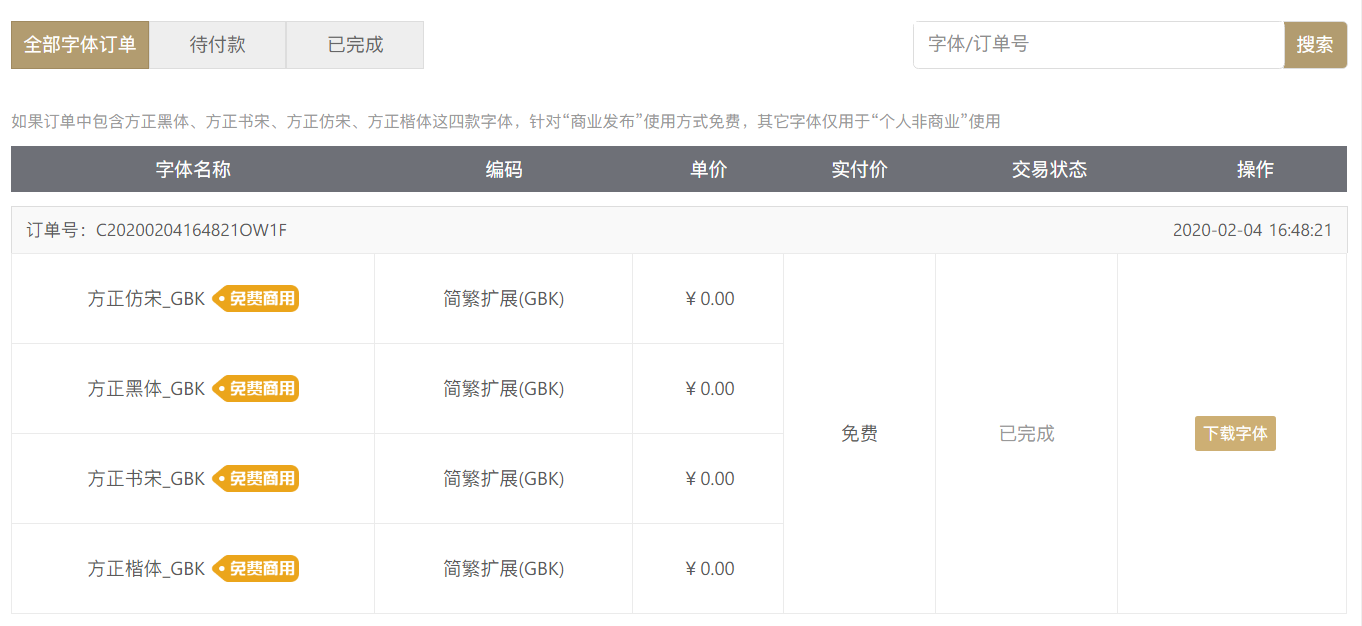
\includegraphics[width=0.9\textwidth]{founder.png}
% \end{figure}

% \subsection{其他中文字体}
% 如果你想完全自定义字体\footnote{这里仍然以方正字体为例。},你可以选择 \lstinline{chinesefont=nofont},然后在导言区设置
% \begin{lstlisting}
% \setCJKmainfont[BoldFont={FZHei-B01},ItalicFont={FZKai-Z03}]{FZShuSong-Z01}
% \setCJKsansfont[BoldFont={FZHei-B01}]{FZKai-Z03}
% \setCJKmonofont[BoldFont={FZHei-B01}]{FZFangSong-Z02}
% \setCJKfamilyfont{zhsong}{FZShuSong-Z01}
% \setCJKfamilyfont{zhhei}{FZHei-B01}
% \setCJKfamilyfont{zhkai}[BoldFont={FZHei-B01}]{FZKai-Z03}
% \setCJKfamilyfont{zhfs}[BoldFont={FZHei-B01}]{FZFangSong-Z02}
% \newcommand*{\songti}{\CJKfamily{zhsong}}
% \newcommand*{\heiti}{\CJKfamily{zhhei}}
% \newcommand*{\kaishu}{\CJKfamily{zhkai}}
% \newcommand*{\fangsong}{\CJKfamily{zhfs}}
% \end{lstlisting}

% \chapter{ElegantBook 写作示例}

% \begin{introduction}
%   \item 积分定义~\ref{def:int}
%   \item Fubini 定理~\ref{thm:fubi}
%   \item 最优性原理~\ref{pro:max}
%   \item 柯西列性质~\ref{property:cauchy}
%   \item 韦达定理
% \end{introduction}

% \section{Lebesgue 积分}
% 在前面各章做了必要的准备后,本章开始介绍新的积分。在 Lebesgue 测度理论的基础上建立了 Lebesgue 积分,其被积函数和积分域更一般,可以对有界函数和无界函数统一处理。正是由于 Lebesgue 积分的这些特点,使得 Lebesgue 积分比 Riemann 积分具有在更一般条件下的极限定理和累次积分交换积分顺序的定理,这使得 Lebesgue 积分不仅在理论上更完善,而且在计算上更灵活有效。

% Lebesgue 积分有几种不同的定义方式。我们将采用逐步定义非负简单函数,非负可测函数和一般可测函数积分的方式。

% 由于现代数学的许多分支如概率论、泛函分析、调和分析等常常用到一般空间上的测度与积分理论,在本章最后一节将介绍一般的测度空间上的积分。

% \subsection{积分的定义}

% 我们将通过三个步骤定义可测函数的积分。首先定义非负简单函数的积分。以下设 $E$ 是 $\mathcal{R}^n$ 中的可测集。

% \begin{definition}[可积性] \label{def:int} 
% 设 $ f(x)=\sum\limits_{i=1}^{k} a_i \chi_{A_i}(x)$ 是 $E$ 上的\textbf{非负简单函数},中文其中 $\{A_1,A_2,\ldots,A_k\}$ 是 $E$ 上的一个可测分割,$a_1,a_2,\ldots,a_k$ 是非负实数。定义 $f$ 在 $E$ 上的积分为 $\int_{a}^b f(x)$
% \begin{equation}
%    \label{inter}
%    \int_{E} f dx = \sum_{i=1}^k a_i m(A_i) \pi \alpha\beta\sigma\gamma\nu\xi\epsilon\varepsilon. \oint_{a}^b\ointop_{a}^b\prod_{i=1}^n
% \end{equation}
% 一般情况下 $0 \leq \int_{E} f dx \leq \infty$。若 $\int_{E} f dx < \infty$,则称 $f$ 在 $E$ 上可积。
% \end{definition}

% 一个自然的问题是,Lebesgue 积分与我们所熟悉的 Riemann 积分有什么联系和区别?在 4.4 在我们将详细讨论 Riemann 积分与 Lebesgue 积分的关系。这里只看一个简单的例子。设 $D(x)$ 是区间 $[0,1]$ 上的 Dirichlet 函数。即 $D(x)=\chi_{Q_0}(x)$,其中 $Q_0$ 表示 $[0,1]$ 中的有理数的全体。根据非负简单函数积分的定义,$D(x)$ 在 $[0,1]$ 上的 Lebesgue 积分为
% \begin{equation}
%    \label{inter2}
%    \int_0^1 D(x)dx = \int_0^1 \chi_{Q_0} (x) dx = m(Q_0) = 0
% \end{equation}
% 即 $D(x)$ 在 $[0,1]$ 上是 Lebesgue 可积的并且积分值为零。但 $D(x)$ 在 $[0,1]$ 上不是 Riemann 可积的。


% 有界变差函数是与单调函数有密切联系的一类函数。有界变差函数可以表示为两个单调递增函数之差。与单调函数一样,有界变差函数几乎处处可导。与单调函数不同,有界变差函数类对线性运算是封闭的,它们构成一线空间。练习题 \ref{exer:43} 是一个性质的证明。

% \begin{exercise}\label{exer:43}
% 设 $f \notin\in L(\mathcal{R}^1)$,$g$ 是 $\mathcal{R}^1$ 上的有界可测函数。证明函数
% \begin{equation}
%    \label{ex:1}
%    I(t) = \int_{\mathcal{R}^1} f(x+t)g(x)dx \quad t \in \mathcal{R}^1
% \end{equation}
% 是 $\mathcal{R}^1$ 上的连续函数。 
% \end{exercise}

% \begin{solution}
% 即 $D(x)$ 在 $[0,1]$ 上是 Lebesgue 可积的并且积分值为零。但 $D(x)$ 在 $[0,1]$ 上不是 Riemann 可积的。
% \end{solution}

% \begin{proof}
% 即 $D(x)$ 在 $[0,1]$ 上是 Lebesgue 可积的并且积分值为零。但 $D(x)$ 在 $[0,1]$ 上不是 Riemann 可积的。
% \end{proof}

% \begin{theorem}[Fubini 定理] \label{thm:fubi} 
% (1)若 $f(x,y)$ 是 $\mathcal{R}^p\times\mathcal{R}^q$ 上的非负可测函数,则对几乎处处的 $x\in \mathcal{R}^p$,$f(x,y)$ 作为 $y$ 的函数是 $\mathcal{R}^q$ 上的非负可测函数,$g(x)=\int_{\mathcal{R}^q}f(x,y) dy$ 是 $\mathcal{R}^p$ 上的非负可测函数。并且
% \begin{equation}
%    \label{eq:461}
%    \int_{\mathcal{R}^p\times\mathcal{R}^q} f(x,y) dxdy=\int_{\mathcal{R}^p}\left(\int_{\mathcal{R}^q}f(x,y)dy\right)dx.
% \end{equation}

% (2)若 $f(x,y)$ 是 $\mathcal{R}^p\times\mathcal{R}^q$ 上的可积函数,则对几乎处处的 $x\in\mathcal{R}^p$,$f(x,y)$ 作为 $y$ 的函数是 $\mathcal{R}^q$ 上的可积函数,并且 $g(x)=\int_{\mathcal{R}^q}f(x,y) dy$ 是 $\mathcal{R}^p$ 上的可积函数。而且~\ref{eq:461} 成立。
% \end{theorem}

% \ref{thm:fubi}

% \begin{note}
% 在本模板中,引理(lemma),推论(corollary)的样式和定理~\ref{thm:fubi} 的样式一致,包括颜色,仅仅只有计数器的设置不一样。
% \end{note}

% 我们说一个实变或者复变量的实值或者复值函数是在区间上平方可积的,如果其绝对值的平方在该区间上的积分是有限的。所有在勒贝格积分意义下平方可积的可测函数构成一个希尔伯特空间,也就是所谓的 $L^2$ 空间,几乎处处相等的函数归为同一等价类。形式上,$L^2$ 是平方可积函数的空间和几乎处处为 0 的函数空间的商空间。

% \begin{proposition}[最优性原理] \label{pro:max}
% 如果 $u^*$ 在 $[s,T]$ 上为最优解,则 $u^*$ 在 $[s, T]$ 任意子区间都是最优解,假设区间为 $[t_0, t_1]$ 的最优解为 $u^*$ ,则 $u(t_0)=u^{*}(t_0)$,即初始条件必须还是在 $u^*$ 上。
% \end{proposition}

% 我们知道最小二乘法可以用来处理一组数据,可以从一组测定的数据中寻求变量之间的依赖关系,这种函数关系称为经验公式。本课题将介绍最小二乘法的精确定义及如何寻求点与点之间近似成线性关系时的经验公式。假定实验测得变量之间的 $n$ 个数据,则在平面上,可以得到 $n$ 个点,这种图形称为 “散点图”,从图中可以粗略看出这些点大致散落在某直线近旁, 我们认为其近似为一线性函数,下面介绍求解步骤。

% \begin{figure}[htbp]
%   \centering
%   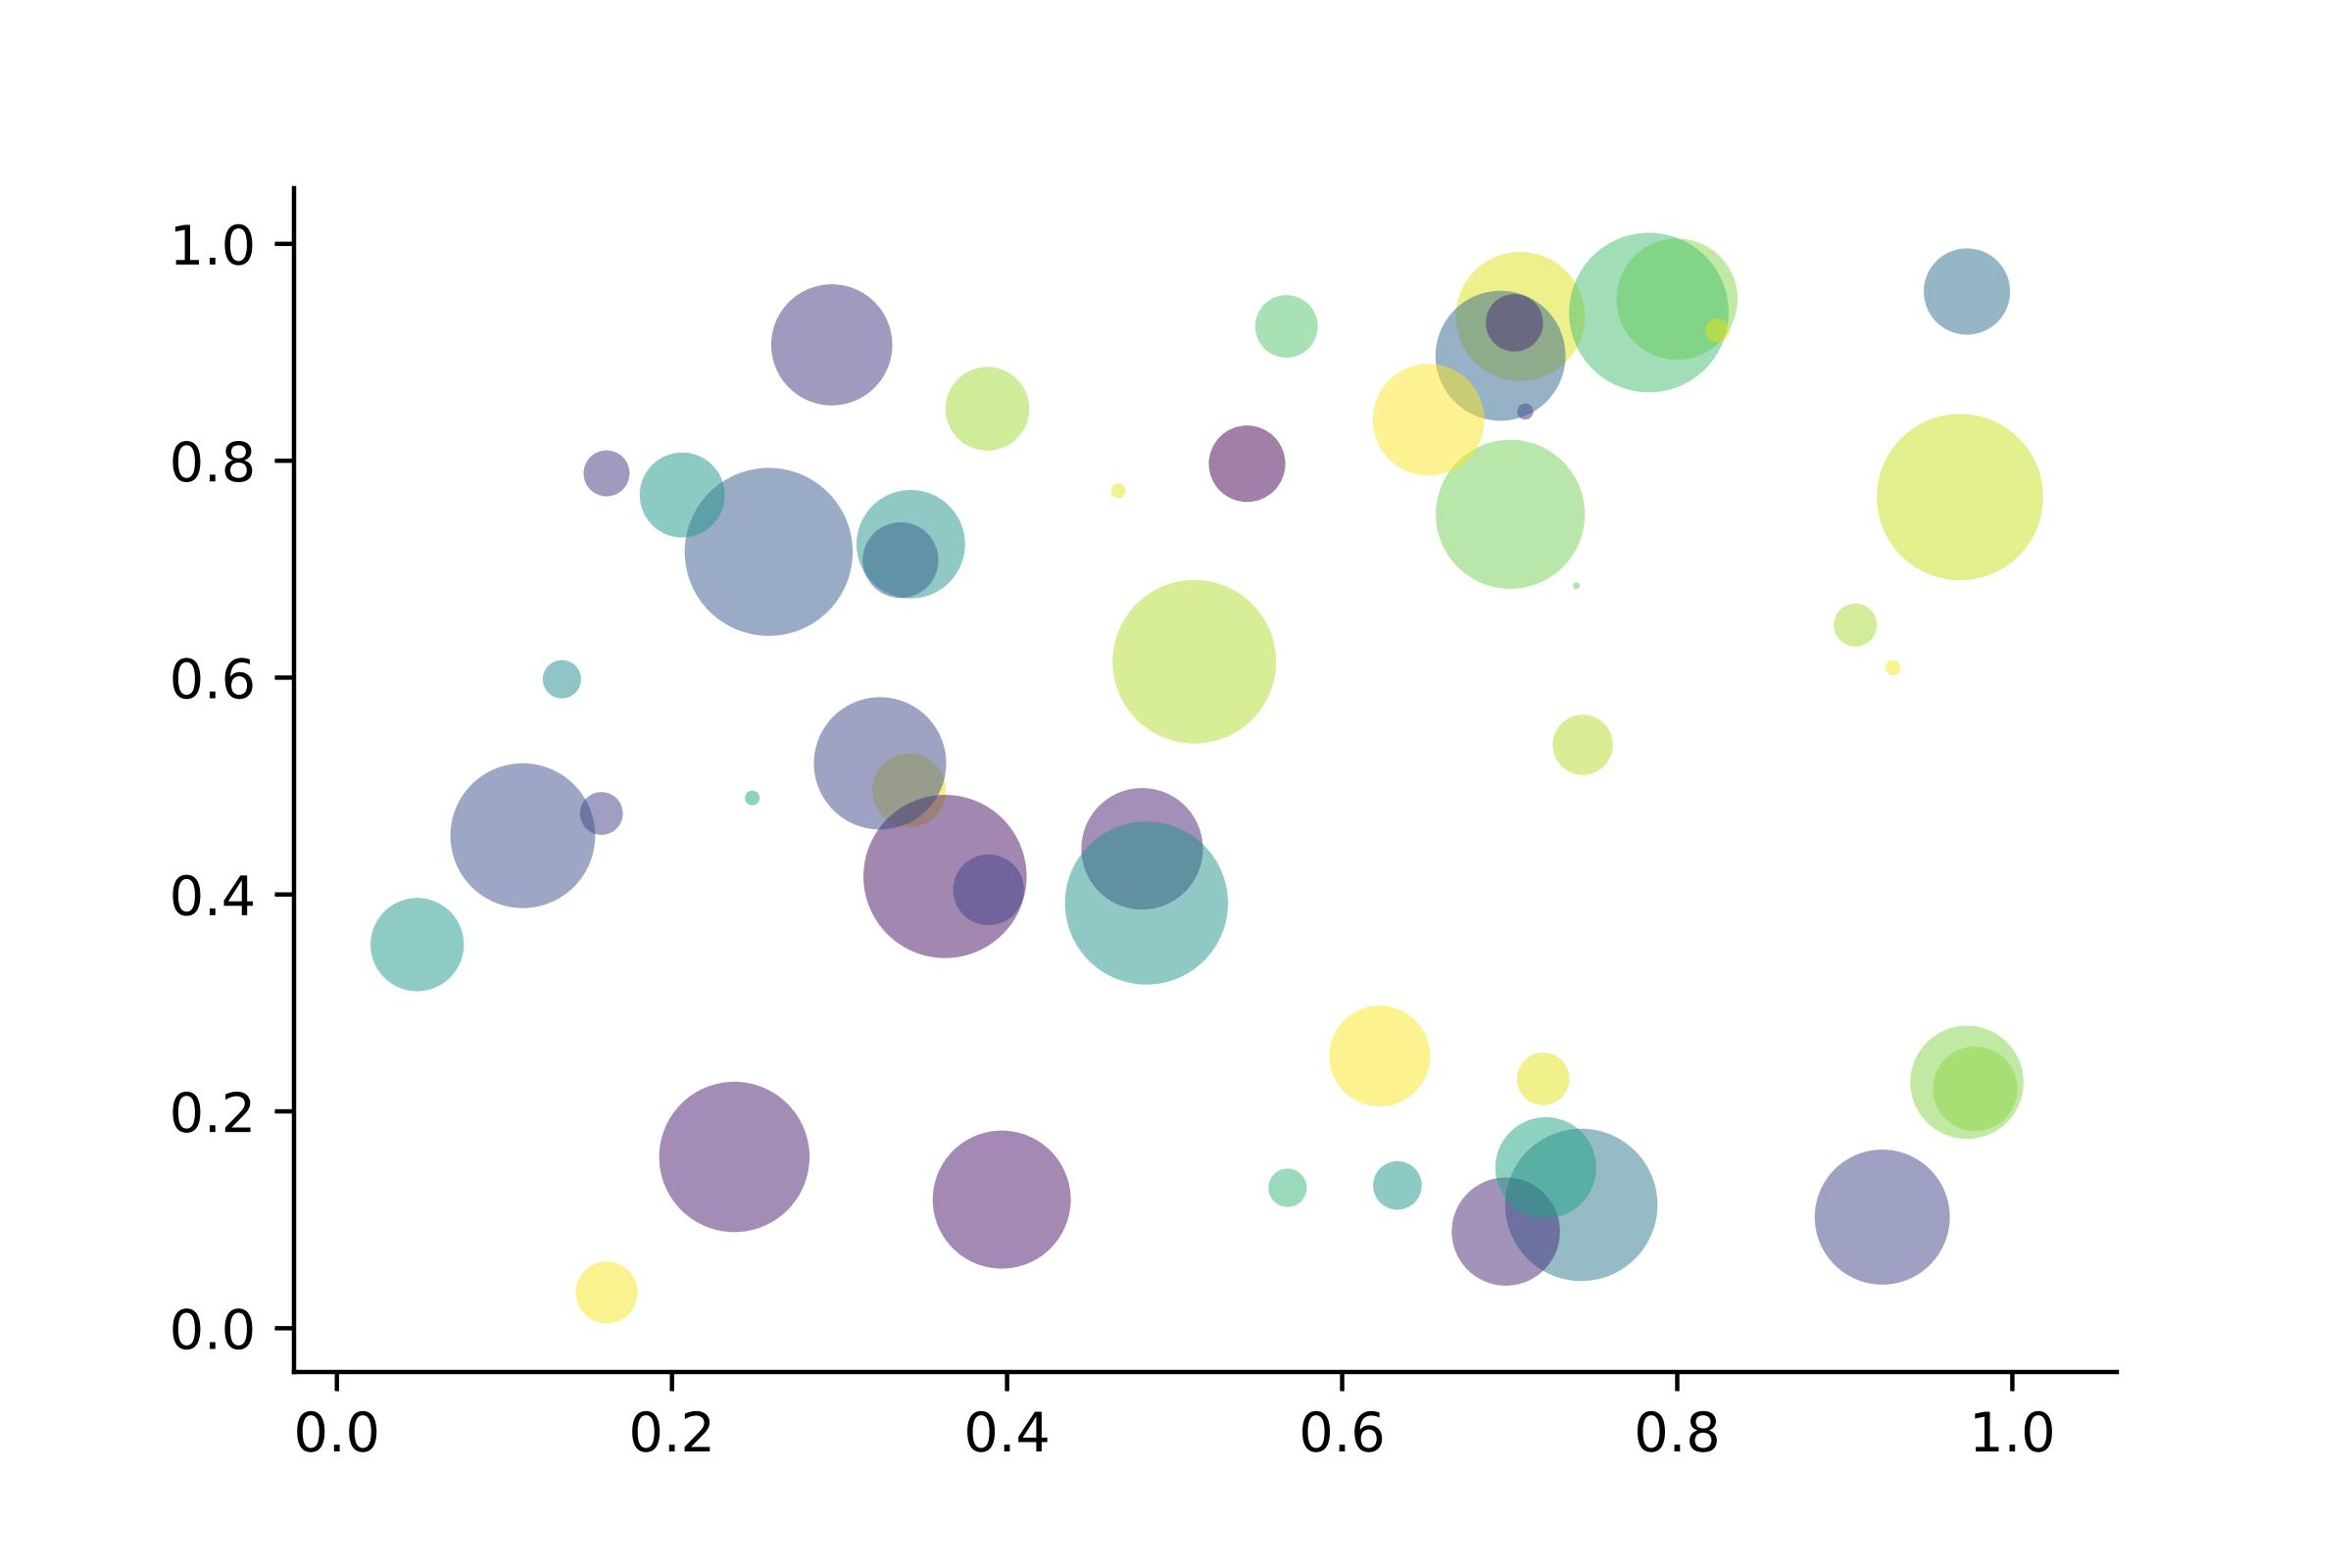
\includegraphics[width=0.6\textwidth]{scatter.jpg}
%   \caption{散点图示例 $\hat{y}=a+bx$ \label{fig:scatter}}
% \end{figure}

% 以最简单的一元线性模型来解释最小二乘法。什么是一元线性模型呢?监督学习中,如果预测的变量是离散的,我们称其为分类(如决策树,支持向量机等),如果预测的变量是连续的,我们称其为回归。回归分析中,如果只包括一个自变量和一个因变量,且二者的关系可用一条直线近似表示,这种回归分析称为一元线性回归分析。如果回归分析中包括两个或两个以上的自变量,且因变量和自变量之间是线性关系,则称为多元线性回归分析。对于二维空间线性是一条直线;对于三维空间线性是一个平面,对于多维空间线性是一个超平面。

% \begin{property}\label{property:cauchy}
% 柯西列的性质
% \begin{enumerate}
% \item $\{x_k\}$ 是柯西列,则其子列 $\{x_k^i\}$ 也是柯西列。
% \item $x_k\in \mathcal{R}^n$,$\rho(x,y)$ 是欧几里得空间,则柯西列收敛,$(\mathcal{R}^n,\rho)$ 空间是完备的。
% \end{enumerate}
% \end{property}

% \begin{conclusion}
% 回归分析(regression analysis) 是确定两种或两种以上变量间相互依赖的定量关系的一种统计分析方法。运用十分广泛,回归分析按照涉及的变量的多少,分为一元回归和多元回归分析;按照因变量的多少,可分为简单回归分析和多重回归分析;按照自变量和因变量之间的关系类型,可分为线性回归分析和非线性回归分析。
% \end{conclusion}

% \begin{problemset}
% \item 设 $A$ 为数域 $K$ 上的 $n$ 级矩阵。证明:如果 $K^n$ 中任意非零列向量都是 $A$ 的特征向量,则 $A$ 一定是数量矩阵。
% \item 证明:不为零矩阵的幂零矩阵不能对角化。
% \item 设 $A = (a_{ij})$ 是数域 $K$ 上的一个 $n$ 级上三角矩阵,证明:如果 $a_{11} = a_{22} = \cdots = a_{nn}$,并且至少有一个 $a_{kl} \not = 0 (k < l)$,则 $A$ 一定不能对角化。
% \end{problemset}

% \chapter{常见问题集}

% 我们根据用户社区反馈整理了下面一些常见的问题,用户在遇到问题时,应当首先查阅本手册和本部分的常见的问题。

% \begin{enumerate}[itemsep=1.5ex]
%   \item \question{有没有办法章节用“第一章,第一节,(一)”这种?}
%     见前文介绍,可以使用 \lstinline{scheme=chinese} 设置。
%   \item \question{大佬,我想把正文字体改为亮色,背景色改为黑灰色。}
%     页面颜色可以使用 \lstinline{\pagecolor} 命令设置,文本命令可以参考\href{https://tex.stackexchange.com/questions/278544/xcolor-what-is-the-equivalent-of-default-text-color}{这里}进行设置。
%   \item \question{\lstinline[breaklines]{Package ctex Error: CTeX fontset 'Mac' is unavailable.}}
%     在 Mac 系统下,中文编译请使用 \hologo{XeLaTeX}。
%   \item \question{\lstinline{! LaTeX Error: Unknown option 'scheme=plain' for package 'ctex'.}}
%     你用的 C\TeX{} 套装吧?这个里面的 \lstinline{ctex} 宏包已经是已经是 10 年前的了,与本模板使用的 \lstinline{ctex} 宏集有很大区别。不建议 C\TeX{} 套装了,请卸载并安装 \TeX{} Live 2022。
%   \item \question{我该使用什么版本?}
%     请务必使用\href{https://github.com/ElegantLaTeX/ElegantBook/releases}{最新正式发行版},发行版间不定期可能会有更新(修复 bug 或者改进之类),如果你在使用过程中没有遇到问题,不需要每次更新\href{https://github.com/ElegantLaTeX/ElegantBook/archive/master.zip}{最新版},但是在发行版更新之后,请尽可能使用最新版(发行版)!最新发行版可以在 GitHub 或者 \TeX{} Live 2021 内获取。
%   \item \question{我该使用什么编辑器?}
%     你可以使用 \TeX{} Live 2021 自带的编辑器 \TeX{}works 或者使用 \TeX{}studio,\TeX works 的自动补全,你可以参考我们的总结 \href{https://github.com/EthanDeng/texworks-autocomplete}{\TeX works 自动补全}。推荐使用 \TeX{} Live 2021 + \TeX{}studio。我自己用 VS Code 和 Sublime Text,相关的配置说明,请参考 \href{https://github.com/EthanDeng/vscode-latex}{\LaTeX{} 编译环境配置:Visual Studio Code 配置简介} 和 \href{https://github.com/EthanDeng/sublime-text-latex}{Sublime Text 搭建 \LaTeX{} 编写环境}。
%   \item \question{您好,我们想用您的 ElegantBook 模板写一本书。关于机器学习的教材,希望获得您的授权,谢谢您的宝贵时间。}
%     模板的使用修改都是自由的,你们声明模板来源以及模板地址(GitHub 地址)即可,其他未尽事宜按照开源协议 LPPL-1.3c。做好之后,如果方便的话,可以给我们一个链接,我把你们的教材放在 Elegant\LaTeX{} 用户作品集里。
%   \item \question{请问交叉引用是什么?}
%     本群和本模板适合有一定 \LaTeX{} 基础的用户使用,新手请先学习 \LaTeX{} 的基础,理解各种概念,否则你将寸步难行。
%   \item \question{代码高亮环境能用其他语言吗?}
%     可以的,ElegantBook 模板用的是 \lstinline{listings} 宏包,你可以在环境(\lstinline{lstlisting})之后加上语言(比如 Python 使用 \lstinline{language=Python} 选项),全局语言修改请使用 \lstinline{lsset} 命令,更多信息请参考宏包文档。
%   \item \question{群主,什么时候出 Beamer 的模板(主题),ElegantSlide 或者 ElegantBeamer?}
%     由于 Beamer 中有一个很优秀的主题 \href{https://github.com/matze/mtheme}{Metropolis}。后续确定不会再出任何主题/模板,请大家根据需要修改已有主题。
% \end{enumerate}

% \chapter{版本更新历史}

% 根据用户的反馈,我们不断修正和完善模板。由于 3.00 之前版本与现在版本差异非常大,在此不列出 3.00 之前的更新内容。


% \datechange{2022/04/09}{版本 4.3 正式发布。}

% \begin{change}
%   \item 放弃 newtx 系列宏包的设置,改用 TeX Gyre Terms,并设置其他字体;
%   \item 修改定理类环境内部字体设置,修复环境内部中文无法加粗问题;
%   \item 增加定理类环境的计数器选项 \lstinline{thmcnt},可选 \lstinline{chapter} 和 \lstinline{section};
%   \item 增加 \lstinline{bibend} 选项,可选 \lstinline{bibend=biber}(默认)和 \lstinline{bibend=bibtex}。
% \end{change}



% \datechange{2022/03/08}{版本 4.2 正式发布。}

% \begin{change}
%   \item 对于 newtx 系列宏包更新导致的字体 bug 的修复;
%   \item 修缮目录格式,为了达到这个目的,重新改写 \lstinline{\chaptername} 的重定义语句;
%   \item 增加日语 \lstinline{lang=jp} 设定。
%   \item 这个版本为一个临时性版本,在 \TeX Live 2022 发布之后,将尽快发布 4.3 版本,由于对于中文的改动比较大,可能会出现预期之外的 bug,有问题可以在 QQ 群或者 Github 反馈。
% \end{change}


% \datechange{2021/05/02}{版本 4.1 正式发布。}

% \begin{change}
%   \item \textbf{重要改动}:由原先的 \hologo{BibTeX} 改为 biblatex 编译方式(后端为 \lstinline{biber}),请注意两者之间的差异;
%   \item \textbf{重要改进}:修改对于定理写法兼容方式,提高数学公式代码的兼容性;
%   \item 页面设置改动,默认页面更宽;方便书写和阅读;
%   \item 支持目录文字以及页码跳转;
%   \item 不再维护 \hologo{pdfLaTeX} 中文支持方式,请务必使用 \hologo{XeLaTeX} 编译中文文稿。
%   \item 增加多个语言选项,法语 \lstinline{lang=fr}、荷兰语 \lstinline{lang=nl}、匈牙利语 \lstinline{lang=hu}、西班牙语 \lstinline{lang=es}、蒙古语 \lstinline{lang=mn} 等。
% \end{change}


% \datechange{2020/04/12}{版本 3.11 正式发布,\textcolor{red}{此版本为 3.x 最后版本。}}

% \begin{change}
%   \item \textbf{重要修正}:修复因为 \lstinline{gbt7714} 宏包更新导致的 \lstinline{natbib option clash} 错误;
%   \item 由于 \lstinline{pgfornament} 宏包未被 \TeX{} Live 2020 收录,因此删除 base 相关的内容;
%   \item 修复部分环境的空格问题;
%   \item 增加了意大利语言选项 \lstinline{lang=it}。
% \end{change}


% \datechange{2020/02/10}{版本 3.10 正式发布}

% \begin{change}
%   \item 增加数学字体选项 \lstinline{math},可选项为 \lstinline{newtx} 和 \lstinline{cm}。\\
%   \textbf{重要提示}:原先通过 \lstinline{newtxmath} 宏包设置的数学字体改为 \LaTeX{} 默认数学字体,如果需要保持原来的字体,需要显式声明数学字体(\lstinline{math=newtx});
%   \item 新增中文字体选项 \lstinline{chinesefont},可选项为 \lstinline{ctexfont}、\lstinline{founder} 和 \lstinline{nofont}。
%   \item 将封面作者信息设置为可选,并且增加自定义信息命令 \lstinline{\bioinfo};
%   \item 在说明文档中增加版本历史,新增 \lstinline{\datechange} 命令和 \lstinline{change} 环境;
%   \item 增加汉化章节选项 \lstinline{scheme},可选项为汉化 \lstinline{chinese};
%   \item 由于 \lstinline{\lvert} 问题已经修复,重新调整 \lstinline{ctex} 宏包和 \lstinline{amsmath} 宏包位置。
%   \item 修改页眉设置,去除了 \lstinline{\lastpage} 以避免 page anchor 问题,加入 \lstinline{\frontmatter}。
%   \item 修改参考文献选项 \lstinline{cite},可选项为数字 \lstinline{numbers}、 作者-年份 \lstinline{authoryear} 以及上标 \lstinline{super}。
%   \item 新增参考文献样式选项 \lstinline{bibstyle},并将英文模式下参考文献样式 \lstinline{apalike} 设置为默认值,中文仍然使用 \lstinline{gbt7714} 宏包设置。
% \end{change}

% \datechange{2019/08/18}{版本 3.09 正式发布}

% \begin{change}
%   \item \lstinline{\elegantpar} 存在 bug,删除 \lstinline{\elegantpar} 命令,建议用户改用 \lstinline{\marginnote} 和 \lstinline{\marginpar} 旁注命令。
%   \item 积分操作符统一更改为 \lstinline{esint} 宏包设置;
%   \item 新增目录选项 \lstinline{toc},可选项为单栏 \lstinline{onecol} 和双栏 \lstinline{twocol};
%   \item 手动增加参考文献选项 \lstinline{cite},可选项为上标形式 \lstinline{super};
%   \item 修正章节习题(\lstinline{problemset})环境。
% \end{change}

% \datechange{2019/05/28}{版本 3.08 正式发布}

% \begin{change}
%   \item 修复 \lstinline{\part} 命令。
%   \item 引入 Note 模板中的 \lstinline{pad} 选项 \lstinline{device=pad}。
%   \item 数学字体加入 \lstinline{mtpro2} 可选项 \lstinline{math=mtpro2},使用免费的 \lstinline{lite} 子集。
%   \item 将参考文献默认显示方式 \lstinline{authoyear} 改为 \lstinline{numbers}。
%   \item 引入旁注命令 \lstinline{\marginpar}(测试)。
%   \item 新增章节摘要环境 \lstinline{introduction}。
%   \item 新增章节习题环境 \lstinline{problemset}。
%   \item 将 \lstinline{\equote} 重命名为 \lstinline{\extrainfo}。
%   \item 完善说明文档,增加致谢部分。
% \end{change}

% \datechange{2019/04/15}{版本 3.07 正式发布}

% \begin{change}
%   \item 删除中英文自定义字体总设置。
%   \item 新增颜色主题,并将原绿色默认主题设置为蓝色 \lstinline{color=blue}。
%   \item 引入隐藏装饰图案选项 \lstinline{base},可选项有显示 \lstinline{show} 和隐藏 \lstinline{hide}。
%   \item 新增定理模式 \lstinline{mode},可选项有简单模式 \lstinline{simple} 和炫彩模式 \lstinline{fancy}。
%   \item 新增隐藏证明、答案等环境的选项 \lstinline{result=noanswer}。
% \end{change}

% \datechange{2019/02/25}{版本 3.06 正式发布}

% \begin{change}
%   \item 删除水印。
%   \item 新封面,新装饰图案。
%   \item 添加引言使用说明。
%   \item 修复双面 \lstinline{twoside}。
%   \item 美化列表环境。
%   \item 增加 \lstinline{\subsubsection} 的设置。
%   \item 将模板拆分成中英文语言模式。
%   \item 使用 \lstinline{lstlisting} 添加代码高亮。
%   \item 增加定理类环境使用说明。
% \end{change}

% \datechange{2019/01/22}{版本 3.05 正式发布}

% \begin{change}
%   \item 添加 \lstinline{xeCJK} 宏包中文支持方案。
%   \item 修复模板之前对 Ti\textit{k}Z 单位的改动。
%   \item 更新 logo 图。
% \end{change}

% \datechange{2019/01/15}{版本 3.04 正式发布}

% \begin{change}
%   \item 格式化模板代码。
%   \item 增加 \lstinline{\equote} 命令。
%   \item 修改 \lstinline{\date}。
% \end{change}

% \datechange{2019/01/08}{版本 3.03 正式发布}

% \begin{change}
%   \item 修复附录章节显示问题。
%   \item 小幅优化封面代码。
% \end{change}

% \datechange{2018/12/31}{版本 3.02 正式发布}

% \begin{change}
%   \item 修复名字系列命令自定义格式时出现的空格问题,比如 \lstinline{\listfigurename}。
%   \item 英文定理类名字改为中文名。
%   \item 英文结构名改为中文。
% \end{change}

% \datechange{2018/12/16}{版本 3.01 正式发布}

% \begin{change}
%   \item 调整 \lstinline{ctex} 宏包。
%   \item 说明文档增加更新内容。
% \end{change}

% \datechange{2018/12/06}{版本 3.00 正式发布}

% \begin{change}
%   \item 删除 \lstinline{mathpazo} 数学字体选项。
%   \item 添加邮箱命令 \lstinline{\mailto}。
%   \item 修改英文字体为 \lstinline{newtx} 系列,另外大型操作符号维持 cm 字体。
%   \item 中文字体改用 \lstinline{ctex} 宏包自动设置。
%   \item 删除 \lstinline{xeCJK} 字体设置,原因是不同系统字体不方便统一。
%   \item 定理换用 \lstinline{tcolobox} 宏包定义,并基本维持原有的定理样式,优化显示效果,支持跨页;定理类名字重命名,如 etheorem 改为 theorem 等等。
%   \item 删去自定义的缩进命令 \lstinline{\Eindent}。
%   \item 添加参考文献宏包 \lstinline{natbib}。
%   \item 颜色名字重命名。
% \end{change}

% \nocite{*}
% \printbibliography[heading=bibintoc, title=\ebibname]
% \appendix

% \chapter{基本数学工具}


% 本附录包括了计量经济学中用到的一些基本数学,我们扼要论述了求和算子的各种性质,研究了线性和某些非线性方程的性质,并复习了比例和百分数。我们还介绍了一些在应用计量经济学中常见的特殊函数,包括二次函数和自然对数,前 4 节只要求基本的代数技巧,第 5 节则对微分学进行了简要回顾;虽然要理解本书的大部分内容,微积分并非必需,但在一些章末附录和第 3 篇某些高深专题中,我们还是用到了微积分。

% \section{求和算子与描述统计量}

% \textbf{求和算子} 是用以表达多个数求和运算的一个缩略符号,它在统计学和计量经济学分析中扮演着重要作用。如果 $\{x_i: i=1, 2, \ldots, n\}$ 表示 $n$ 个数的一个序列,那么我们就把这 $n$ 个数的和写为:

% \begin{equation}
% \sum_{i=1}^n x_i \equiv x_1 + x_2 +\cdots + x_n
% \end{equation}

\printbibliography[heading=bibintoc, title=\ebibname]
\appendix

\end{document}
